%%% ----- general packages and settings ----- %%%
\documentclass[a4paper, ngerman, bibliography=totoc]{scrreprt}  %%, listof=totoc
\usepackage[T1]{fontenc}
\usepackage[utf8]{inputenc}
\usepackage{lmodern}
\usepackage{babel}
\usepackage{float}
\usepackage{microtype} % fixes line breaks

%%% ----- bibliography ----- %%%
\usepackage[babel, german=quotes]{csquotes}
\usepackage[backend=biber, style=alphabetic-verb]{biblatex}
\bibliography{literatur}
\DeclareFieldFormat[article]{title}{#1\isdot} % http://golatex.de/formatierung-des-literaturverzeichnisses-mit-biblatex-t3988.html

%%% ----- references (http://tex.stackexchange.com/a/83051) ----- %%%
\usepackage{varioref}
\usepackage[breaklinks]{hyperref}
\usepackage{cleveref}
\crefname{lstlisting}{Quelltext}{Quelltext}

%%% ----- listings ----- %%%
\usepackage{xcolor} % http://tex.stackexchange.com/a/150377
\usepackage{listings}
\renewcommand{\lstlistingname}{Quelltext}
\renewcommand*{\lstlistlistingname}{Quelltextverzeichnis}

\definecolor{strings}{rgb}{0.69, 0.196, 0.267}
\definecolor{comments}{rgb}{0.247, 0.518, 0.173}
\definecolor{keywords}{rgb}{0.114, 0.180, 0.992}
\definecolor{linenumbers}{rgb}{0.25, 0.25, 0.25}
\definecolor{linebreakmarker}{rgb}{0.25, 0.25, 0.25}

\lstset{ %
  belowcaptionskip=1\baselineskip{},
  breaklines=true,
  postbreak=\mbox{\textcolor{linebreakmarker}{$\hookrightarrow$}\space},
  captionpos=b,
  commentstyle=\color{comments},
  keywordstyle=\color{keywords}\bfseries,
  morecomment=[s][\color{comments}]{/**}{*/},
  numbers=left,
  numbersep=16pt,
  numberstyle=\tiny\color{linenumbers},
  stringstyle=\color{strings},
  tabsize=2
}

\definecolor{bluekeywords}{rgb}{0.13,0.13,1}
\definecolor{greencomments}{rgb}{0,0.5,0}
\definecolor{redstrings}{rgb}{0.9,0,0}

\lstset{language=[Sharp]C,
  showspaces=false,
  showtabs=false,
  breaklines=true,
  showstringspaces=false,
  breakatwhitespace=true,
  escapeinside={(*@}{@*)},
  commentstyle=\color{greencomments},
  keywordstyle=\color{bluekeywords},
  stringstyle=\color{redstrings},
  basicstyle=\ttfamily,
  numberstyle=\tiny\color{linenumbers},
  morekeywords={ var, abstract, event, new, struct,
  as, explicit, null, switch,
  base, extern, object, this,
  bool, false, operator, throw,
  break, finally, out, true,
  byte, fixed, override, try,
  case, float, params, typeof,
  catch, for, private, uint,
  char, foreach, protected, ulong,
  checked, goto, public, unchecked,
  class, if, readonly, unsafe,
  const, implicit, ref, ushort,
  continue, in, return, using,
  decimal, int, sbyte, virtual,
  default, interface, sealed, volatile,
  delegate, internal, short, void,
  do, is, sizeof, while,
  double, lock, stackalloc,
  else, long, static,
  enum, namespace, string}
}

%%% ----- graphics ----- %%%
\usepackage{graphicx}

%%% ----- fix underscore problems ----- %%%
\usepackage[strings]{underscore}

%%% ----- prevent word breaks ----- %%%
\hyphenation{ECMAScript}

%%% ----- custom commands ----- %%%
% - circled numbers (http://tex.stackexchange.com/a/7045)
\usepackage{tikz}
\newcommand*\circled[1]{\tikz[baseline=(char.base)]{\node[shape=circle,draw,inner sep=2pt] (char) {#1};}}
% - z.B. (http://latex.hpfsc.de/content/latex_tipps_und_tricks/eigene_kommandos/)
\newcommand{\zB}{z.\,B. }

% TEMPORARY FIX: https://tex.stackexchange.com/questions/83440/inputenc-error-unicode-char-u8-not-set-up-for-use-with-latex
\DeclareUnicodeCharacter{00A0}{ }


%%% ---------- Document Data ----------
\title{WEA5\\Hurace.Web}
\author{Bauer, Daniel}
\date{\today}

\begin{document}
\maketitle
\setcounter{page}{1}
\tableofcontents
\chapter{Umfang und Aufwand}
Der Implementierungaufwand beträgt 40 Stunden.\\
Bis auf die optionale Rennanalyse wurden alle Anforderungen umgesetzt.
\chapter{Technologien}
Die Webanwendung \emph{Hurace.Web} wurde wie gefordert mit dem SPA-Framework \emph{Angular} (in der Version 8.2) entwickelt.
Um die Entwicklung zu vereinfachen wurden außerdem folgende externe Bibliotheken verwendet:

\section{Angular Material}
\emph{Angular Material}\footnote{\url{https://material.angular.io/}} bietet Angular-Komponenten (\zB Formularelemente, Navigationsleiste, Lade-Anzeige, ...) im Material-Design von Google an.
Da auch die Desktopanwendung von Hurace im Material-Design gestaltet wurde, ergibt die erneute Verwendung in der Webanwendung ein einheitliches Design für den Benutzer.

\section{ngxs}
\emph{ngxs}\footnote{\url{https://www.ngxs.io/}} ist eine Zustandsverwaltungs-Bibliothek die nach dem CQRS-Muster entworfen und ähnlich zu \emph{Redux}\footnote{\url{https://redux.js.org/}} bzw. \emph{ngrx}\footnote{\url{https://ngrx.io/}} aufgebaut ist.
Durch den Einsatz von \emph{ngxs} kann die Logik zum Laden oder Verändern von Daten (anstatt in den Komponenten) in einen (bzw. mehrere) Service ausgelagert werden, der den Applikationszustand managet.
Da der Applikationszustand nur zentral verändert werden kann können Zustandsveränderungen einfacher verstanden und analysiert werden.

\section{Auth0}
\emph{Auth0}\footnote{\url{https://auth0.com/}} kümmert sich um das Authentifizieren in der Webanwendung.

\section{SignalR}
\emph{SignalR}\footnote{\url{https://dotnet.microsoft.com/apps/aspnet/signalr}} wird eingesetzt damit Echtzeitdaten eines Liverennens, wie aktuelle LäuferIn und Zwischenzeiten, vom ASP.NET-Core-Server an die Webanwendung übertragen werden können.
Dadurch muss die Webanwendung nicht alle \emph{n} Sekunden nachfragen, ob es schon neue Zwischenzeiten für ein Rennen gibt, sondern wird automatisch benachrichtigt.

\chapter{Aufbau}
Der Quellcode wurde in folgende Bereiche strukturiert:

\section{Komponenten}
Der \emph{components}-Ordner beinhaltet alle definierten Angular-Komponenten.
Dabei wurde darauf geachtet das diese möglichst modular und einfach gehalten wurden.
Durch den Einsatz von \emph{ngxs} konnte die Fehlerbehandlung und die Geschäftslogik einfach in entsprechende \emph{state}-Services ausgelagert werden.

\section{Modelle}
Der \emph{dtos}-Ordner beinhaltet die Modeldefinitionen von Daten die von der \emph{Hurace.Api} abgefragt werden.
Die Abkürzung \emph{dto} steht dabei für \emph{DataTransferObject}.
Der \emph{enums}- bzw. \emph{models}-Ordner beinhaltet zusätzliche Modeldefinitionen und Enumerationen.

\section{Hurace.Api Dienste}
Der \emph{services}-Ordner beinhaltet Dienste zum Abfragen von Daten der \emph{Hurace.Api}.
Die \emph{LiveService}-Klasse, die als Singleton in der Webanwendung gestartet wird, kümmert sich um die \emph{SinglaR}-Verbindung zum \emph{Hurace.Api}-Server.

\section{Zustandsverwaltung}
Die Zustandsverwaltung der Webanwendung wurde mit der externen Bibliothek \emph{ngxs} gelöst.
Im \emph{actions}-Ordner werden alle Aktionen definiert die den Applikationszustand verändern können.
Aktionen sind als einfache Klassen abgebildet, wie in-\cref{lst:SkierActions} zu sehen.

\begin{lstlisting}[caption={Definieren einer Aktion}, label=lst:SkierActions]
export class GetAllSkiers {
    static readonly type = '[Skier] GetAll';
}
\end{lstlisting}

Eine Aktion kann anschließend über den \emph{store}-Service, der von \emph{ngxs} bereitgestellt wird, in einer Angular-Komponente (\zB SkierListComponent) ausgelöst werden (\cref{lst:DispatchAction}).

\begin{lstlisting}[caption={Auslösen einer Skier-Aktion}, label=lst:DispatchAction]
constructor(private store: Store) { }
ngOnInit() {
    this.store.dispatch(new GetAllSkiers());
}
\end{lstlisting}

Die Services im \emph{states}-Ordner behandeln die ausgelösten Ereignisse und können einen definierten Applikationszustand \emph{initialState} über die \emph{context.patchState}-Methode verändern (\cref{lst:SkierState}).
Die \emph{@Action}-Annotation wird von \emph{ngxs} bereitgestellt und verbindet die Aktion mit der Behandlungsmethode.
Die Methode \emph{skierService.getAll()} lädt alle SkirennläuferInnen über die \emph{Hurace.Api}.

\begin{lstlisting}[caption={Behandeln einer Skier-Aktion}, label=lst:SkierState]
const initialState: SkierStateModel = {
    all: empty(),
    selected: empty()
};

@Action(GetAllSkiers)
getAllSkier(context: Context) {
    context.patchState({ all: loading() });

    return this.skierService.getAll().pipe(
        tap(skiers => context.patchState({ all: data(skiers) })),
        catchError(e => context.patchState({ all: error(e) }))
    );
}
\end{lstlisting}

Damit die Angular-Komponente, die das Ereignis ausgelöst hat die Änderungen (Liste an SkirennläuferInnen) mitbekommt kann auf den Applikationszustand gehört werden (\cref{lst:subscribe}).

\begin{lstlisting}[caption={Hören auf Zustandsänderungen}, label=lst:subscribe]
constructor(private store: Store) {
    store.select(s => s.skier.all)
        .subscribe(skiers => {
            // skier list changed
        });
}
\end{lstlisting}

Über die Browsererweiterung \emph{Redux DevTools} können außerdem alle Zustandsänderungen der jeweiligen Ereignisse verfolgt werden.
Voraussetzung ist die Registrierung der \emph{Redux DevTools} im Angular-Module mittels \emph{NgxsReduxDevtoolsPluginModule.forRoot()}.
\cref{fig:reduxDevTools} zeigt den Applikationszustand nach Laden eines Skierläufers.
\begin{figure}[H]
    \centering
    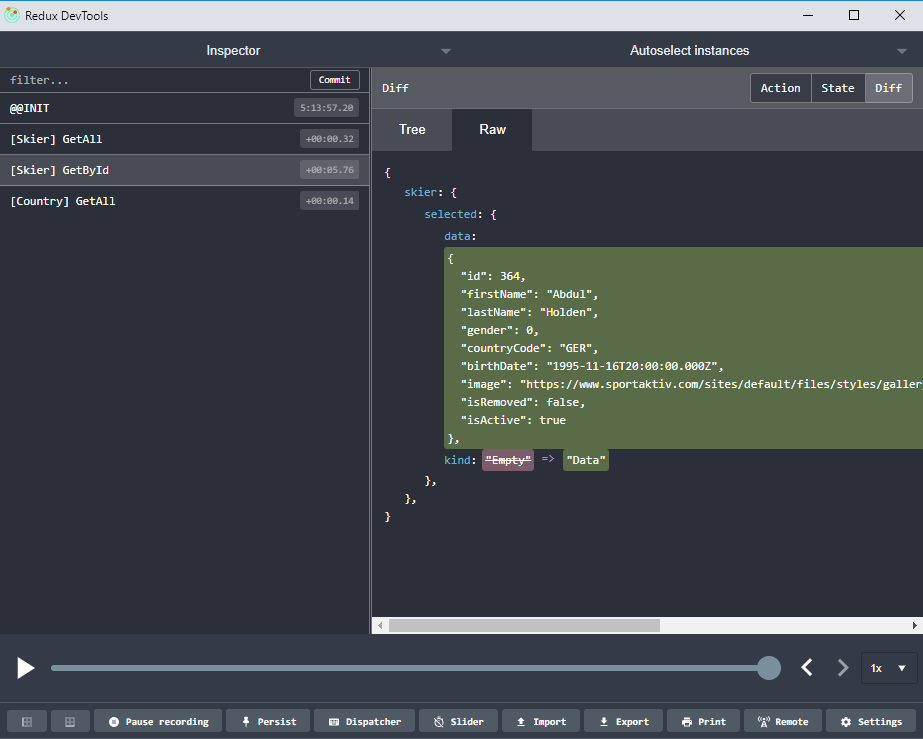
\includegraphics[width=0.9\linewidth]{images/redux-dev-tool}
    \caption{Browsererweiterung Redux DevTools}
\label{fig:reduxDevTools}
\end{figure}

\chapter{Seiten}
Die Webanwendung ist in drei Bereiche gegliedert:
\begin{description}
    \item[Skiers:] Die \emph{Skiers}-Seite zeigt eine Liste von allen SkirennläuferInnen und Detailansicht einer ausgewählten SkirennläuferIn.
    \item[Races:] Die \emph{Races}-Seite zeigt eine Liste von allen Rennen nach Datum sortiert und Detailansicht eines ausgewählten Rennens.
    \item[Season:] Die \emph{Season}-Seite zeigt eine Liste von Rennen, die in der ausgewählten Saison stattfanden.
\end{description}

\section{Skiers}
Die Webanwendung zeigt standardmäßig die \emph{Skiers}-Seite an, in der eine Liste an allen SkirennläuferInnen zu sehen ist (\cref{fig:skiers-list}).
\begin{figure}[H]
    \centering
    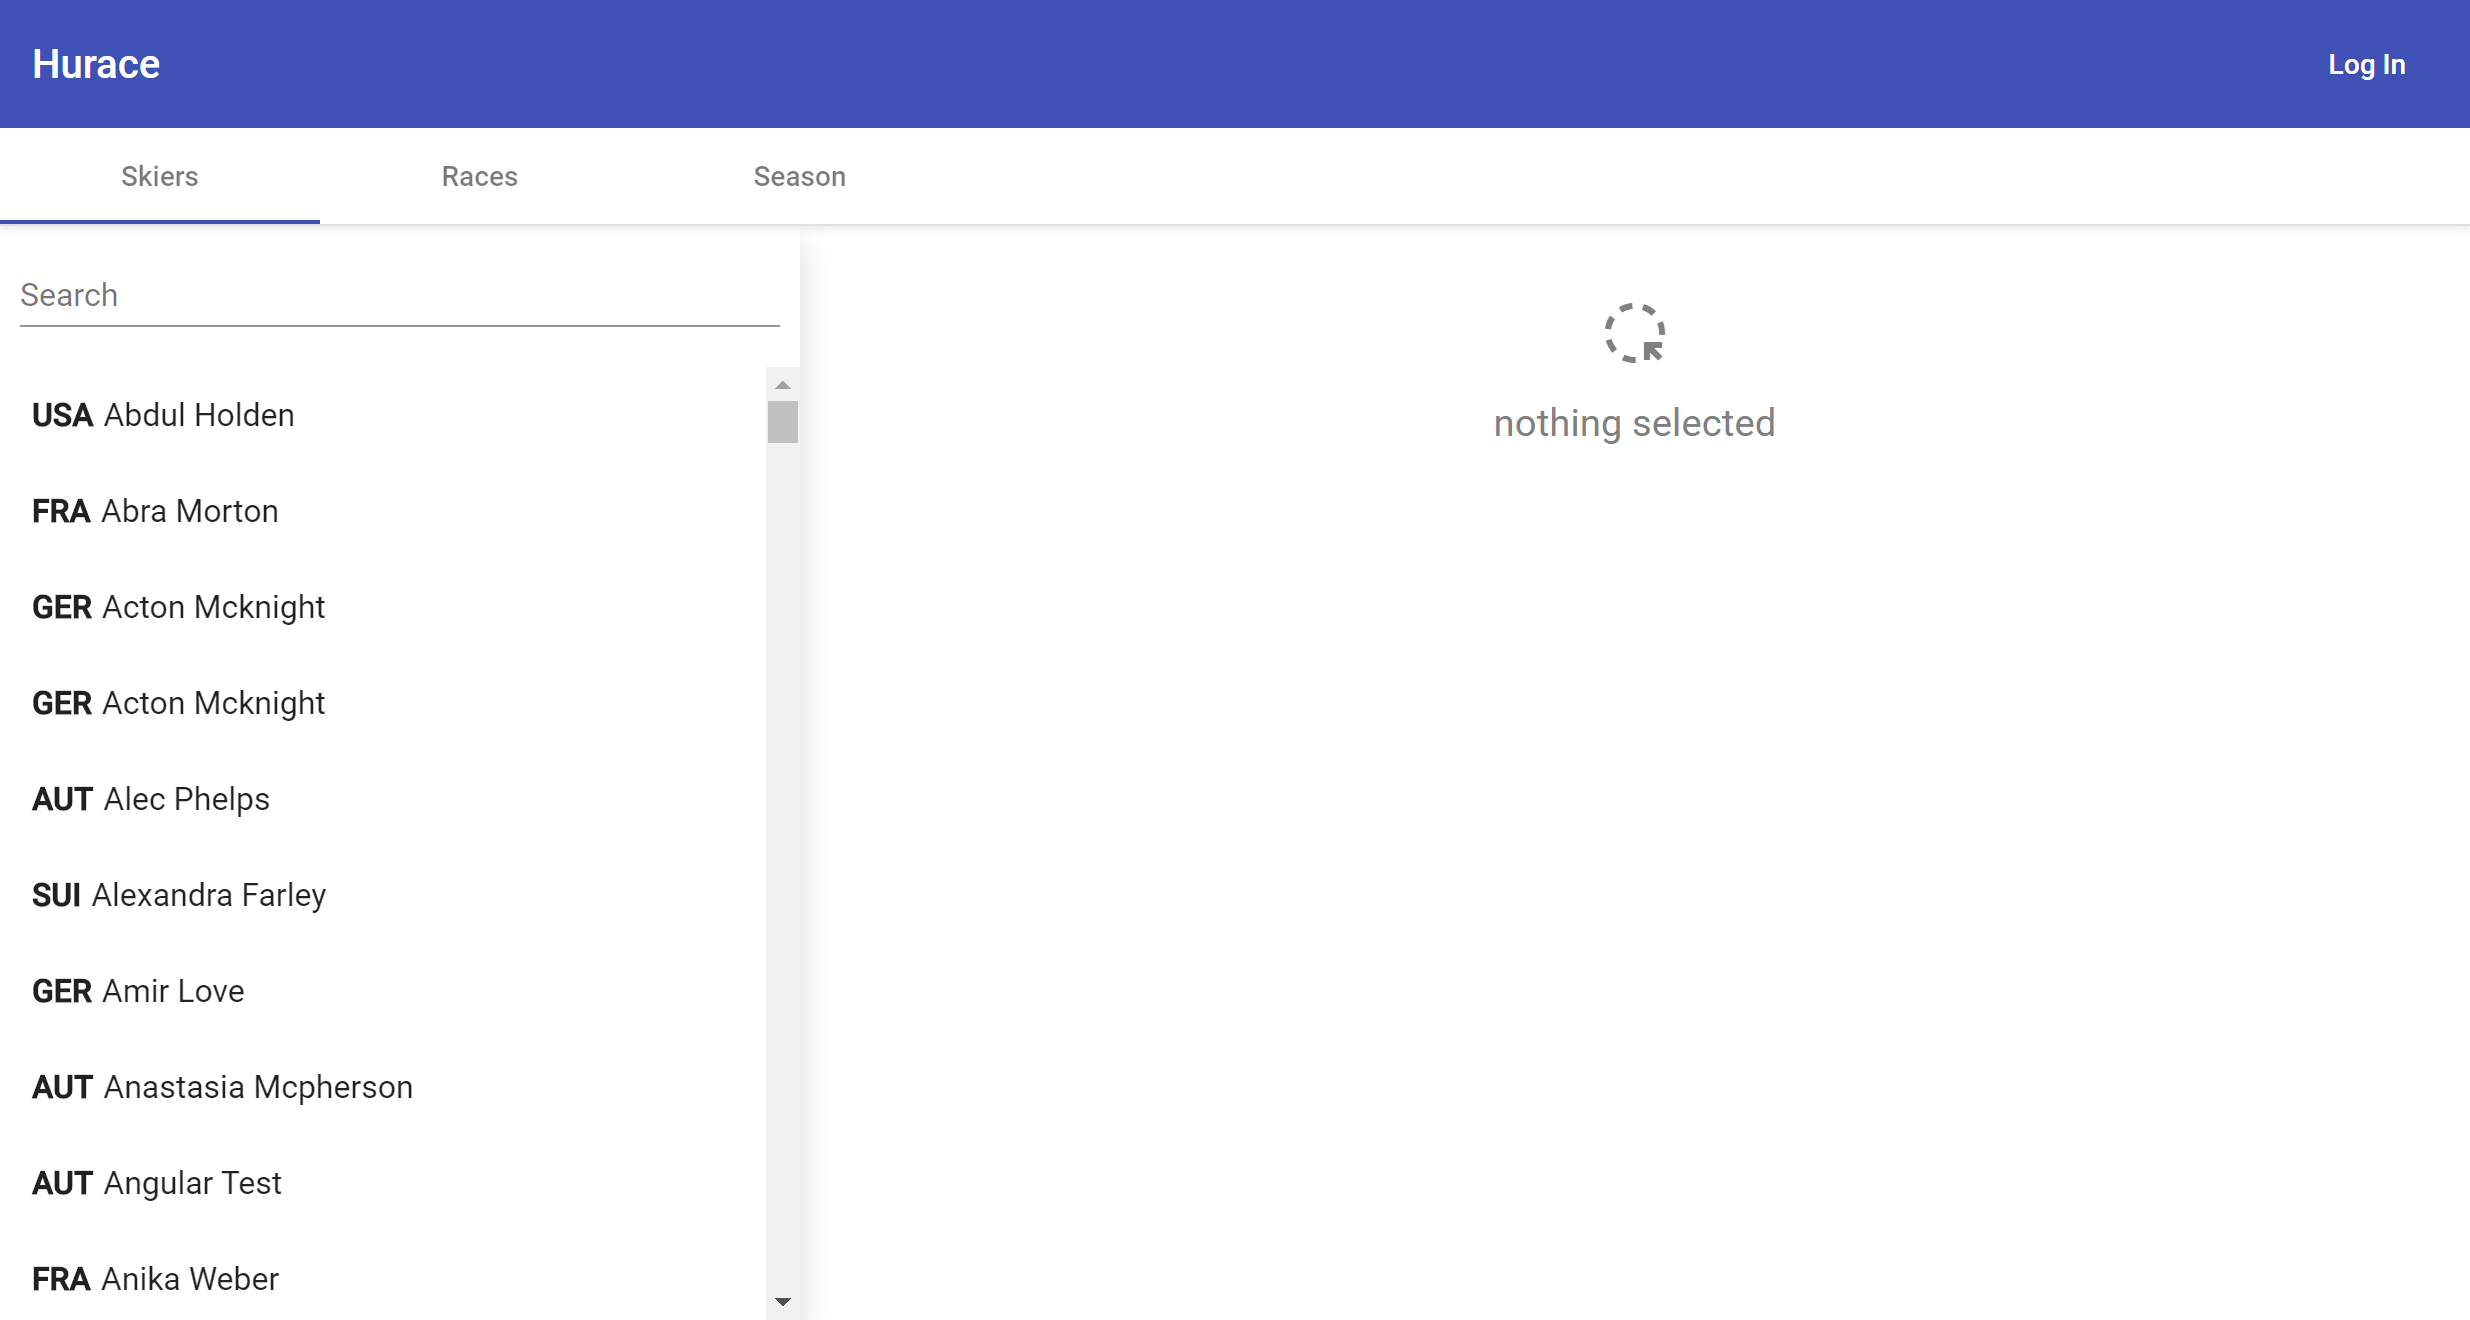
\includegraphics[width=0.9\linewidth]{images/skiers-list}
    \caption{Liste an SkirennläuferInnen}
\label{fig:skiers-list}
\end{figure}

Im Suchfeld kann nach Name oder Länderkürzel (\zB AUT, GER, ...) gefiltert werden (\cref{fig:skiers-search-success}).
\begin{figure}[H]
    \centering
    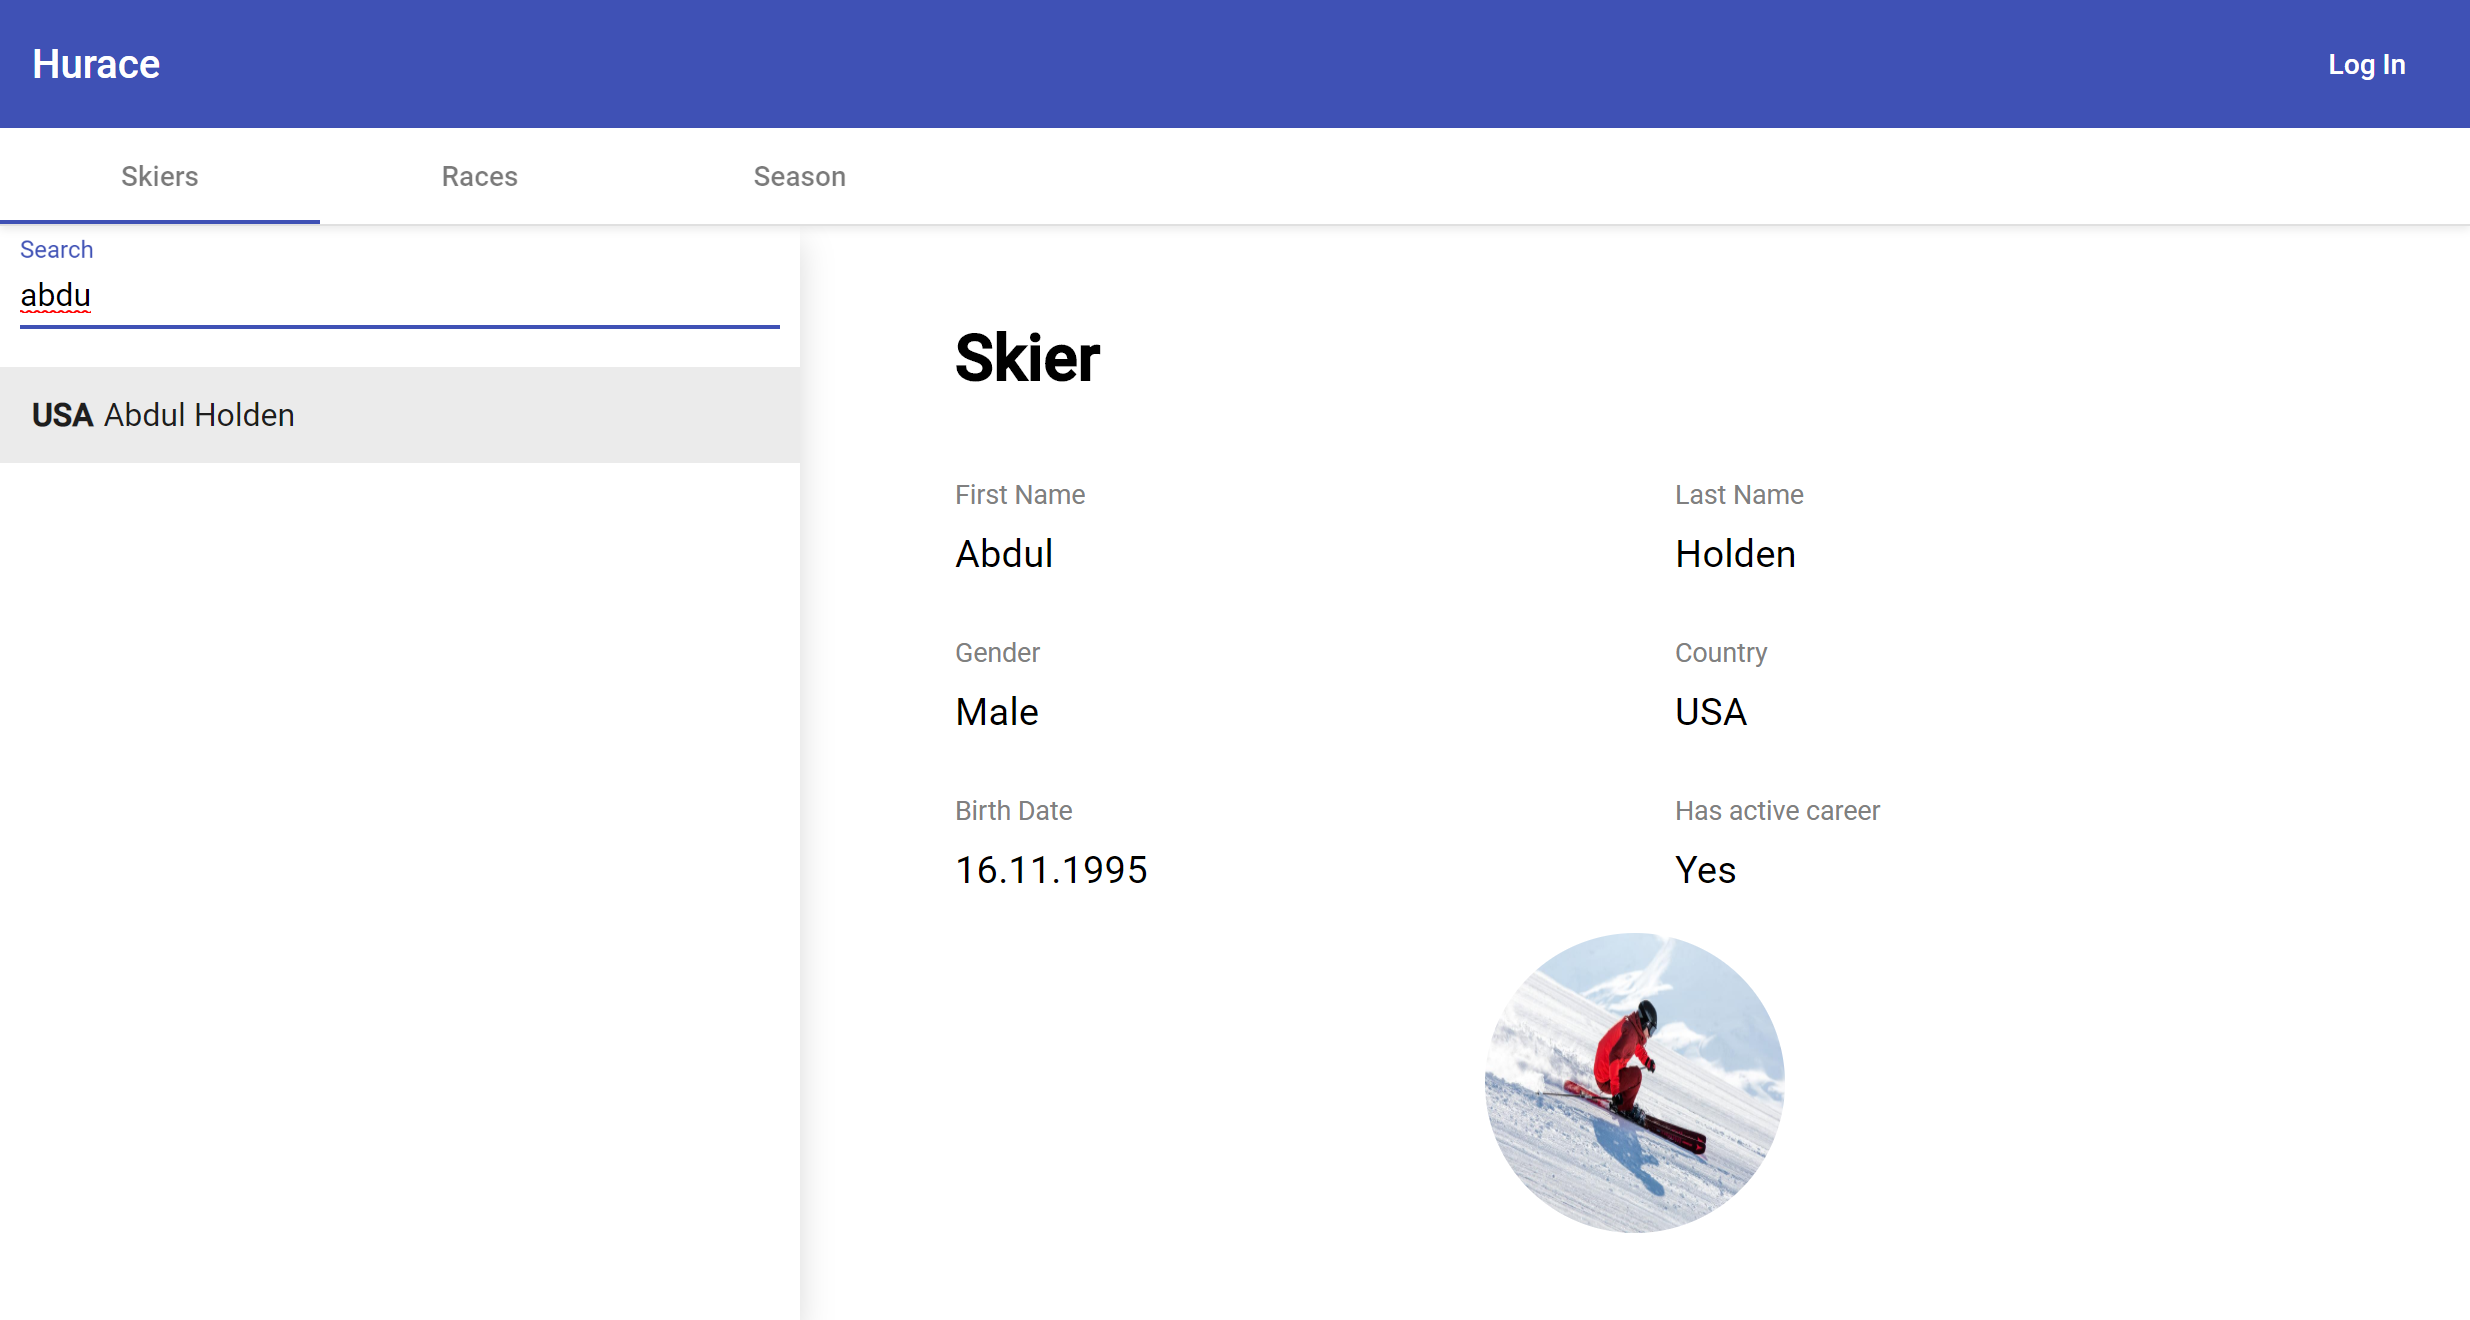
\includegraphics[width=0.9\linewidth]{images/skiers-search-success}
    \caption{Filtern der SkirennläuferInnen}
\label{fig:skiers-search-success}
\end{figure}

Wenn keine SkirennläuferIn gefunden wird wird eine entsprechende Meldung angezeigt (\cref{fig:skiers-search-error}).
\begin{figure}[H]
    \centering
    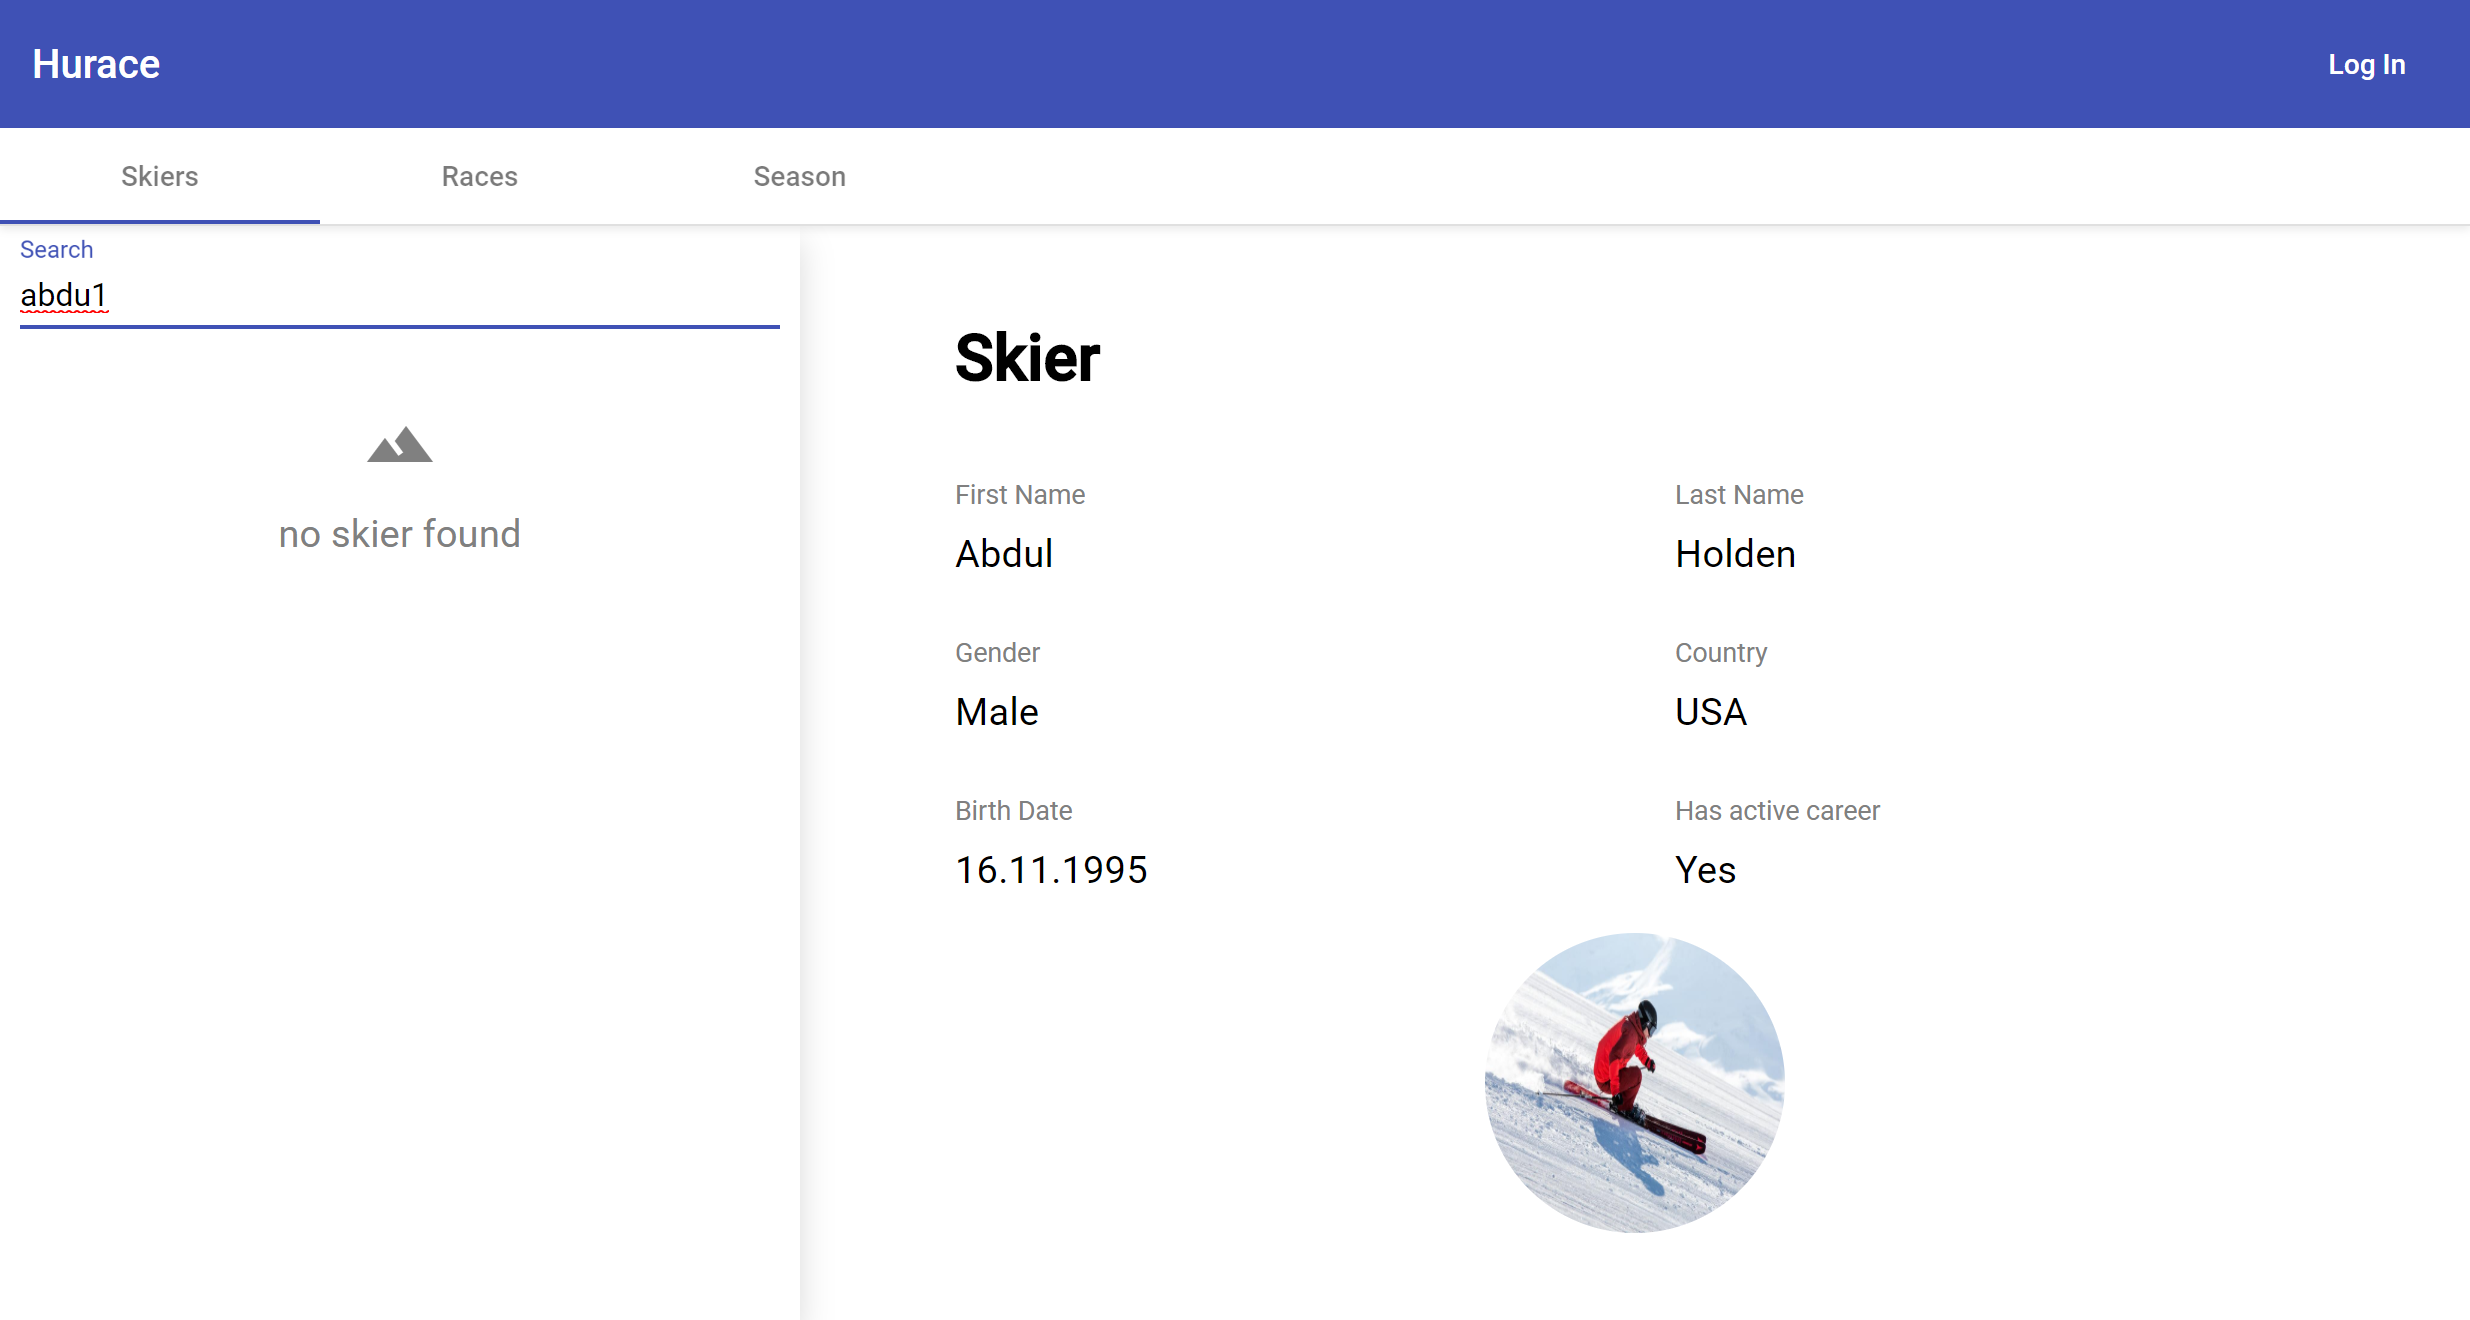
\includegraphics[width=0.9\linewidth]{images/skiers-search-error}
    \caption{Keine Ergebnisse beim Filtern der SkirennläuferInnen}
\label{fig:skiers-search-error}
\end{figure}

Beim Selektieren einer SkirennläuferIn werden weitere Daten angezeigt (\cref{fig:skiers-detail}).
Außerdem ändert sich die Browser-URL auf \emph{/skiers/:id}, sodass bei einem Neuladen die zuvor selektierte SkirennläuferIn angezeigt wird.
\begin{figure}[H]
    \centering
    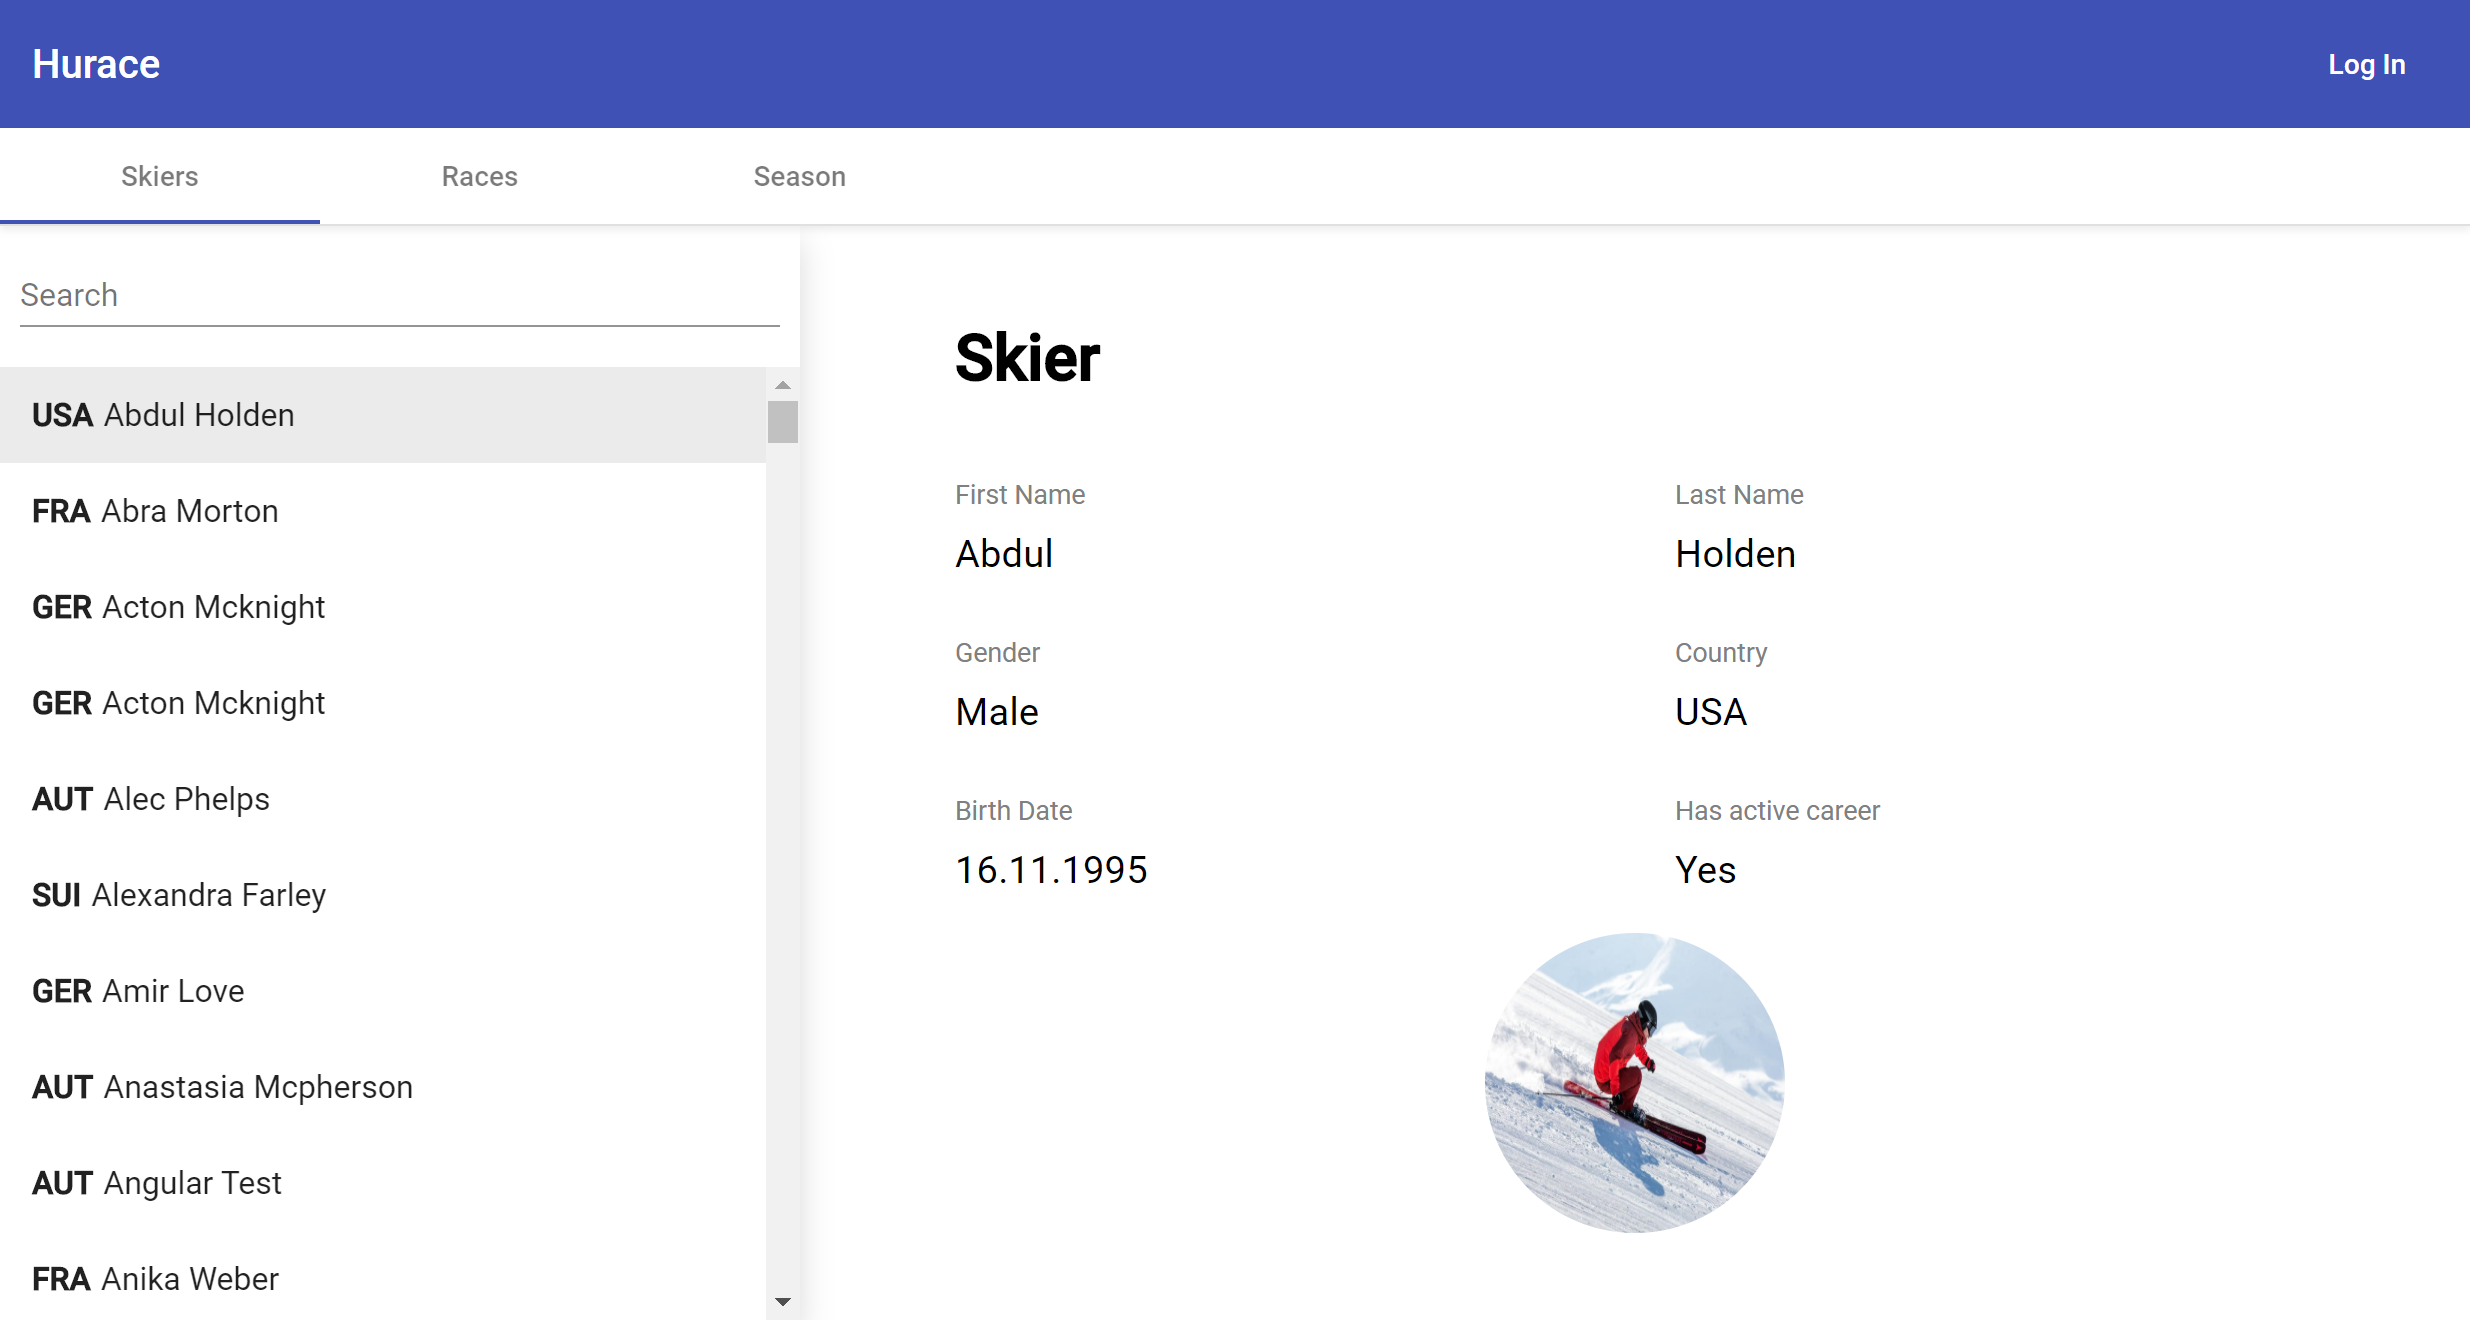
\includegraphics[width=0.9\linewidth]{images/skiers-detail}
    \caption{Detailansicht eines Skirennläufer}
\label{fig:skiers-detail}
\end{figure}

Falls der Anwender angemeldet ist können auch die SkirennläuferInnen bearbeitet oder gelöscht werden (\cref{fig:skiers-form}).
Außerdem können neue SkirennläuferInnen über die \emph{New}-Schaltfläche hinzugefügt werden.
\begin{figure}[H]
    \centering
    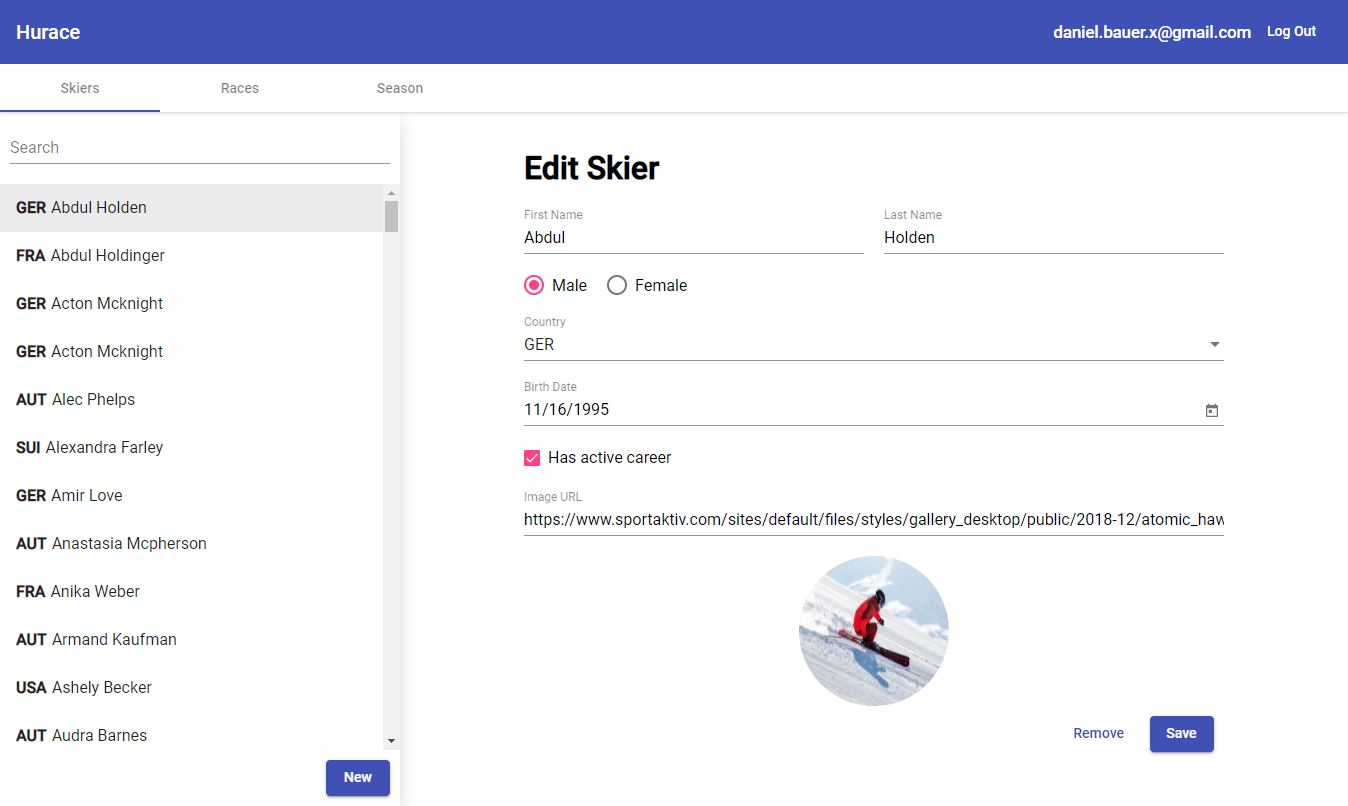
\includegraphics[width=0.9\linewidth]{images/skiers-form}
    \caption{Stammdatenverwaltung eines Skirennläufers}
\label{fig:skiers-form}
\end{figure}

\section{Races}
Die \emph{Races}-Seite zeigt eine Liste von allen Rennen nach Datum sortiert an (\cref{fig:races-list}).
\begin{figure}[H]
    \centering
    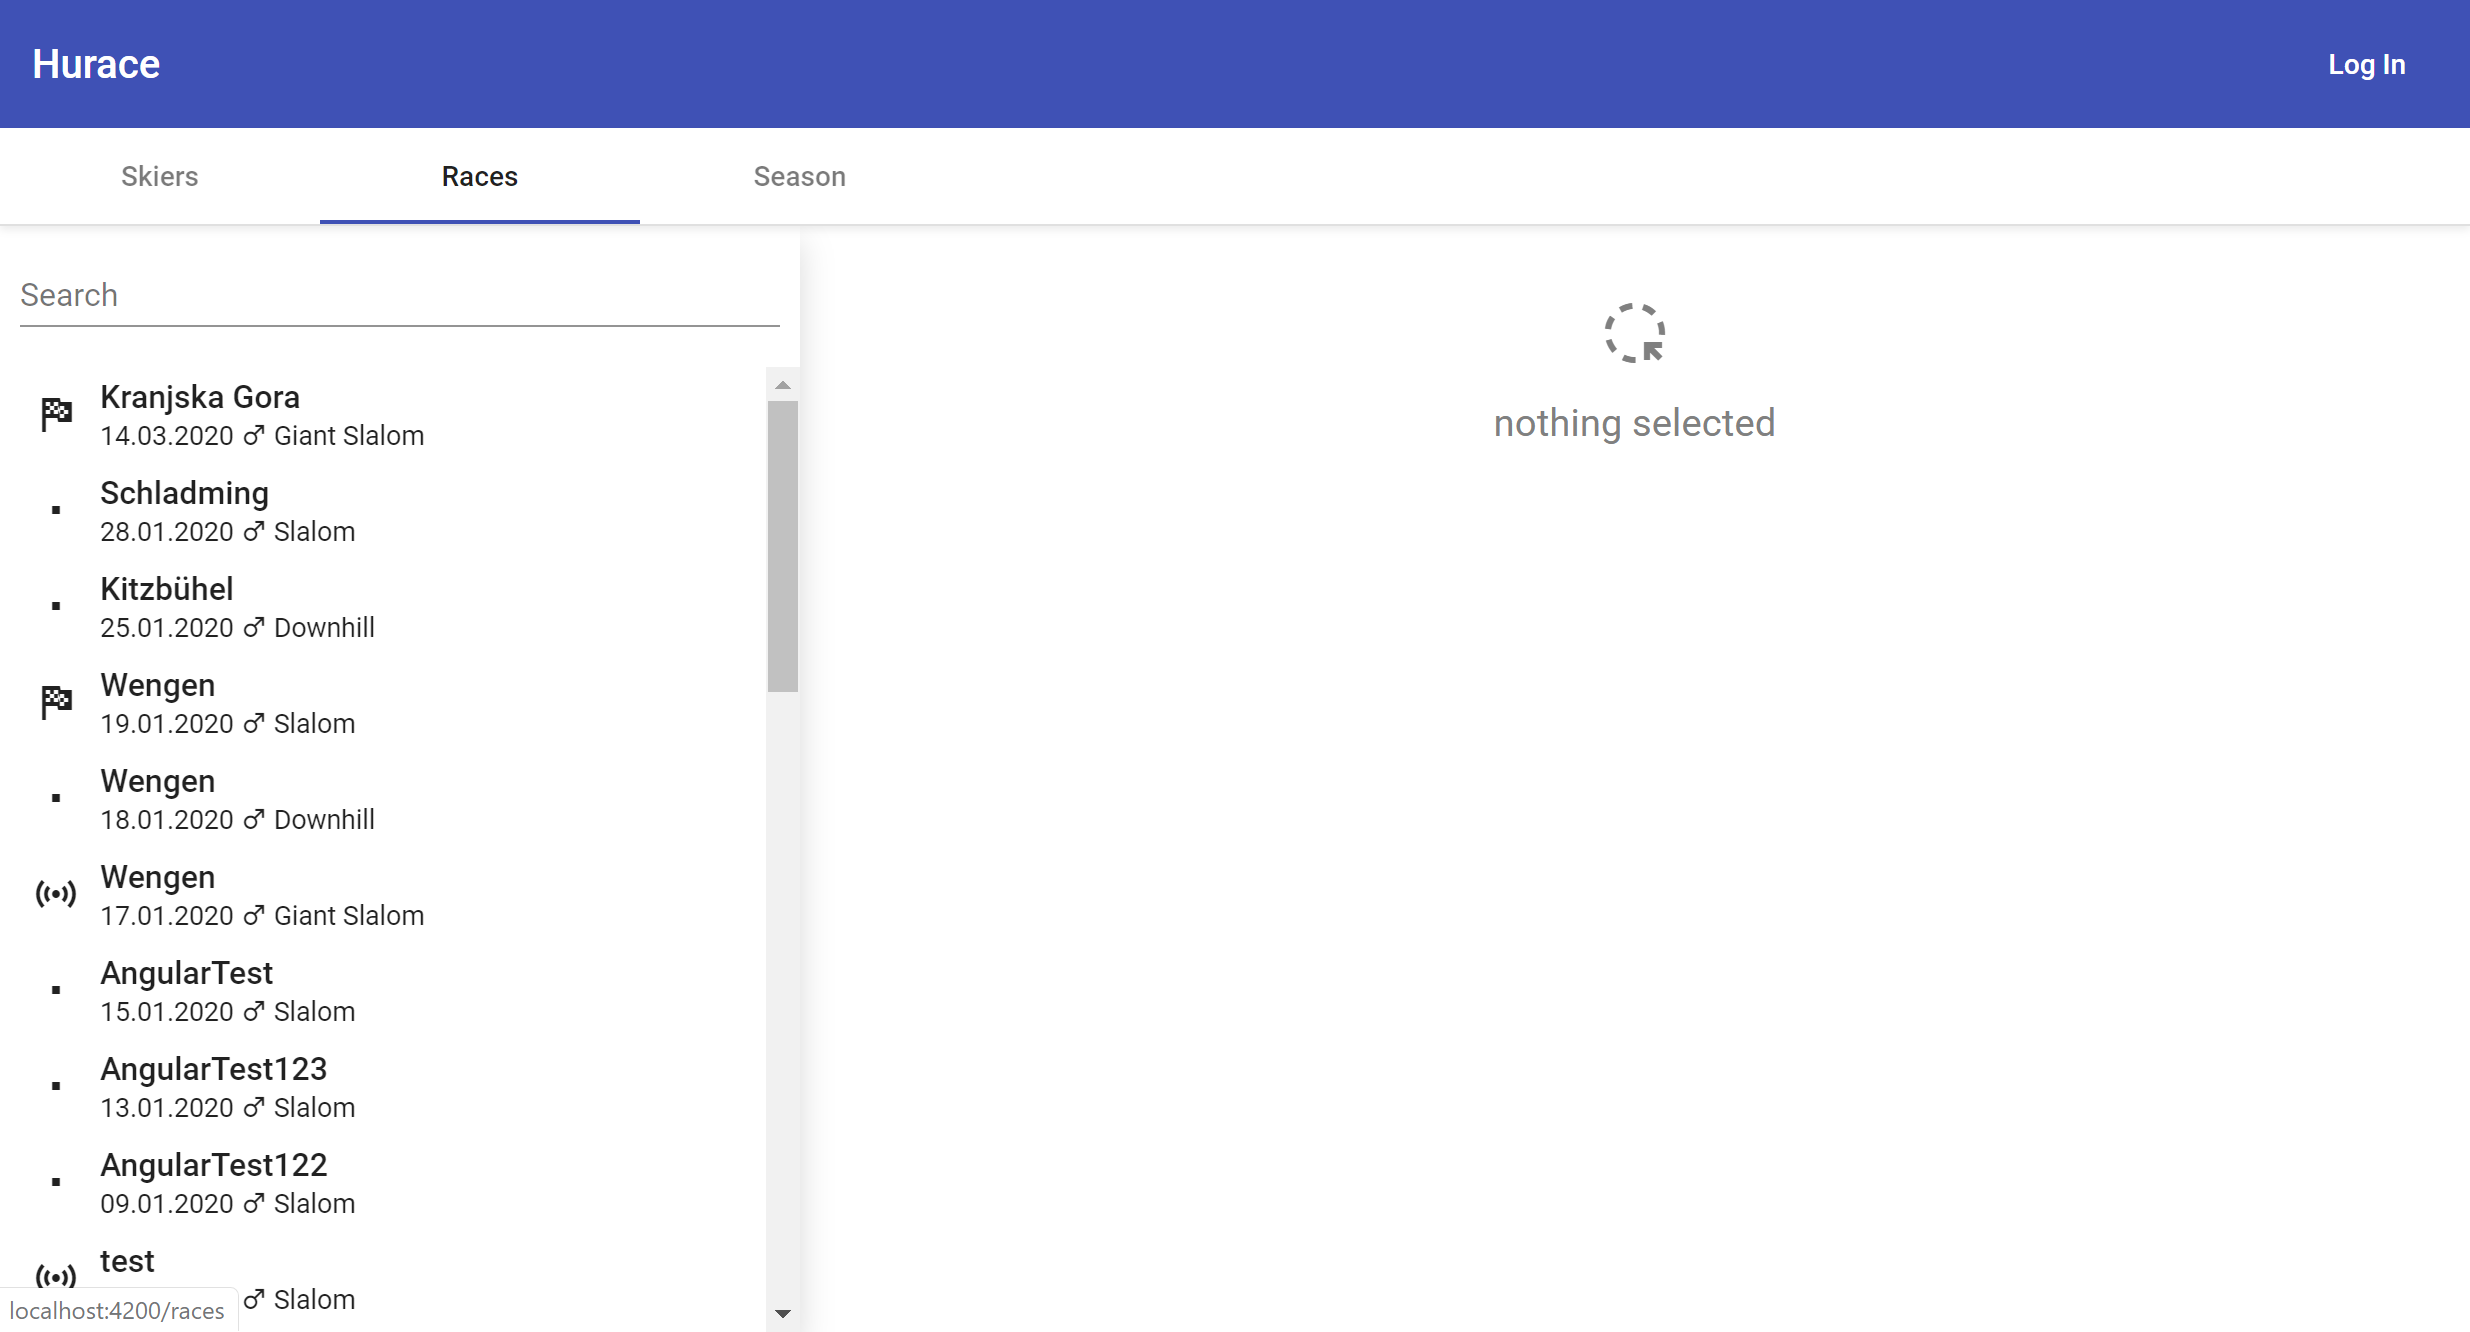
\includegraphics[width=0.9\linewidth]{images/races-list}
    \caption{Liste an Rennen}
\label{fig:races-list}
\end{figure}

Im Suchfeld kann nach Name gefiltert werden (\cref{fig:races-search-success}).
\begin{figure}[H]
    \centering
    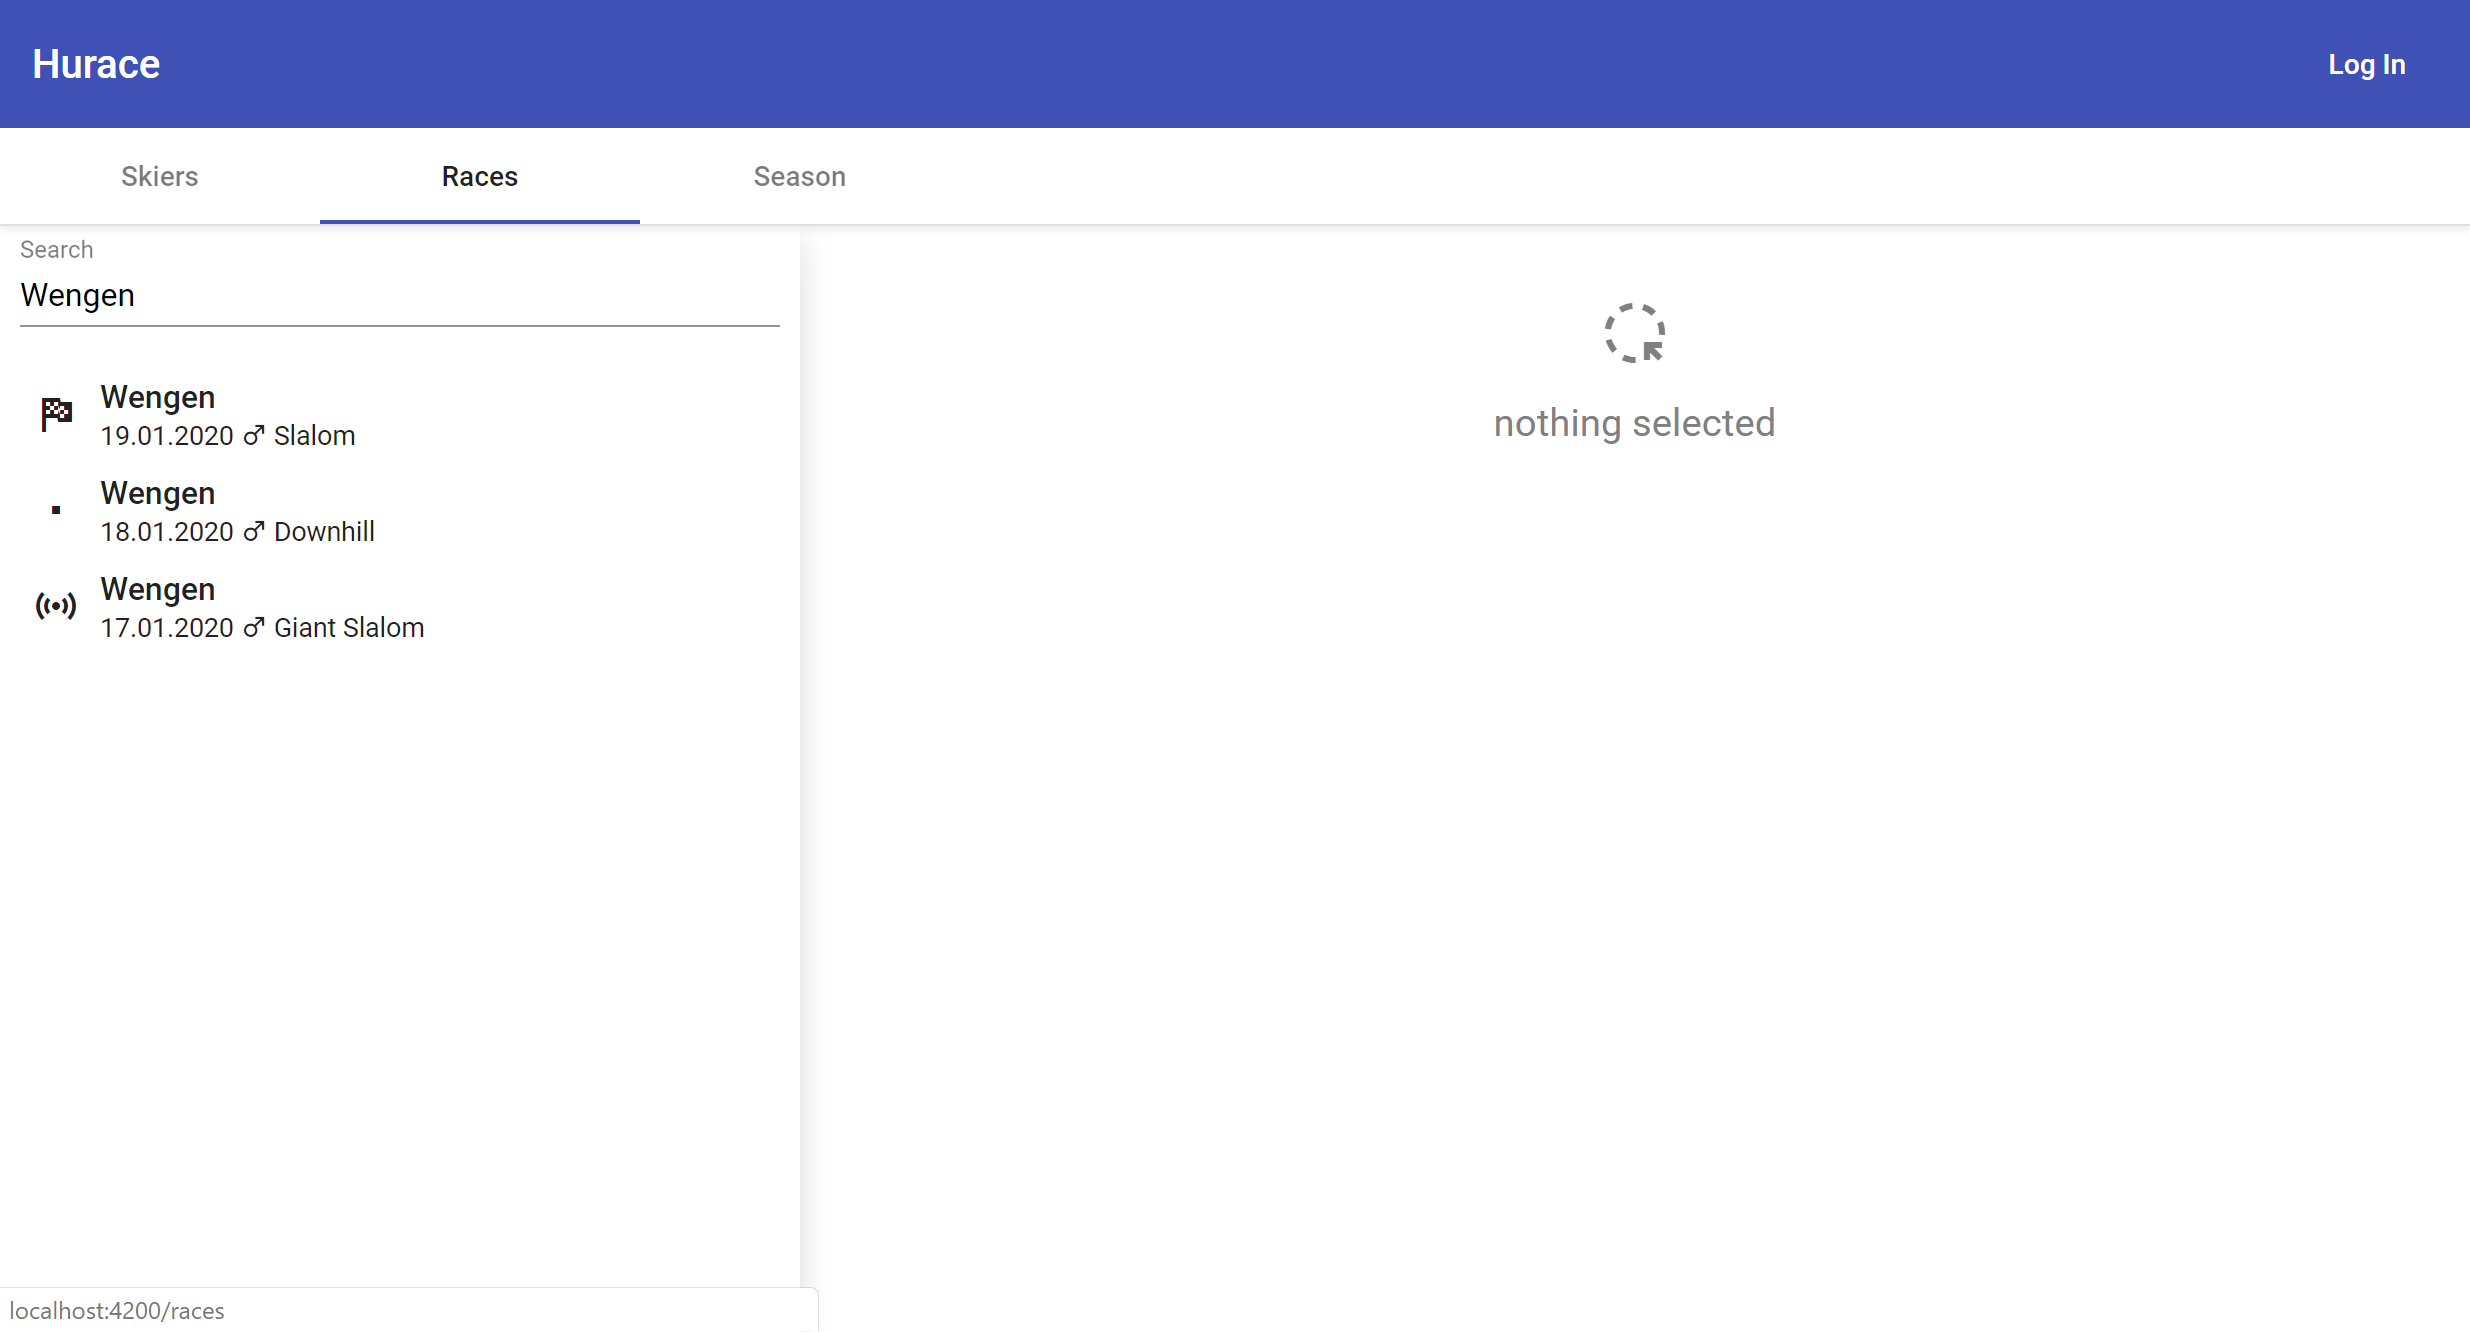
\includegraphics[width=0.9\linewidth]{images/races-search-success}
    \caption{Filtern der Rennen}
\label{fig:races-search-success}
\end{figure}

Wenn kein Rennen gefunden wird, wird eine entsprechende Meldung angezeigt (\cref{fig:races-search-error}).
\begin{figure}[H]
    \centering
    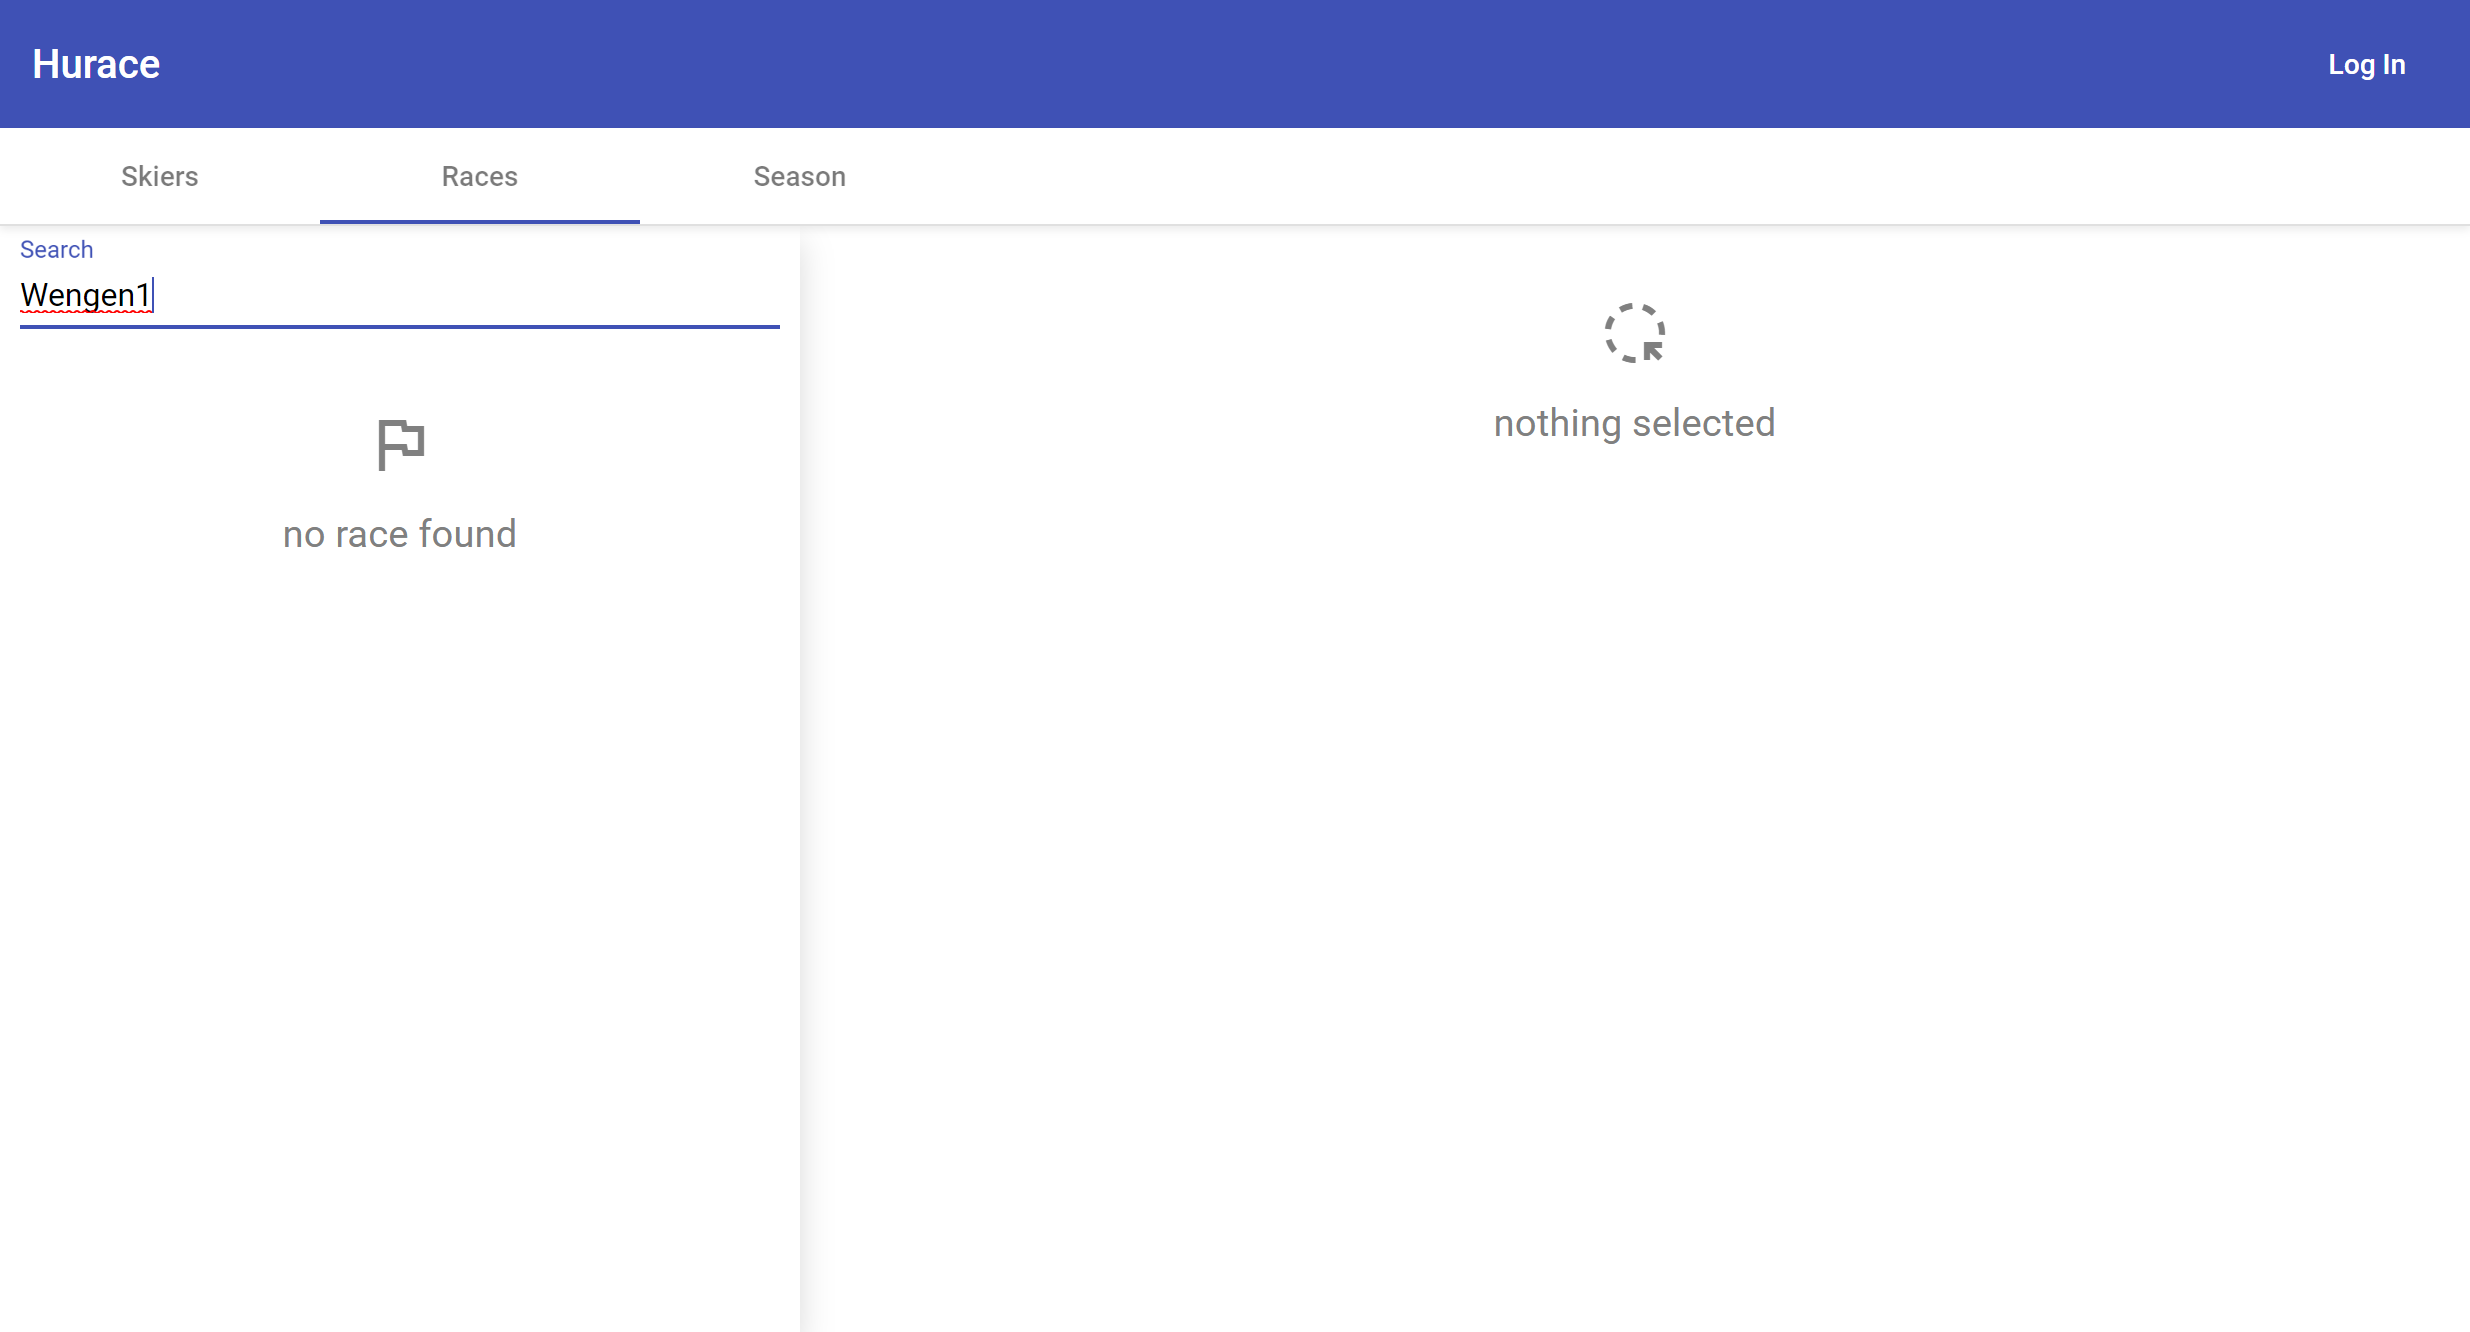
\includegraphics[width=0.9\linewidth]{images/races-search-error}
    \caption{Keine Ergebnisse beim Filtern der Rennen}
\label{fig:races-search-error}
\end{figure}

Beim Selektieren eines Rennens werden weitere Detaildaten angezeigt (\cref{fig:races-detail}).
Außerdem ändert sich die Browser-URL auf \emph{/races/:id}, sodass bei einem Neuladen das zuvor selektierte Rennen angezeigt wird.
Je nach Rennstatus werden unterschiedliche Detaildaten angezeigt:

\begin{description}
    \item[Abgeschlossenes Rennen:] Es werden die Endergebnisse der Durchgänge angezeigt. Bei Rennen mit zwei Durchgänge kann auch der Zwischenstand des ersten Durchgangs angsehen werden (\cref{fig:races-detail}).
    \item[Laufendes Rennen:] Bei einem laufendem Rennen wird zusätzlich zu den Ergebnissen die aktuelle SkirennläuferIn und deren Zwischenzeiten angezeigt (\cref{fig:races-live}).
    \item[Nicht gestartetes Rennen:] Der Benutzer wird mit der Meldung vertröstet, dass das Rennen erst zu einem späteren Zeitpunkt stattfindet (\cref{fig:races-not-started}).
\end{description}

\begin{figure}[H]
    \centering
    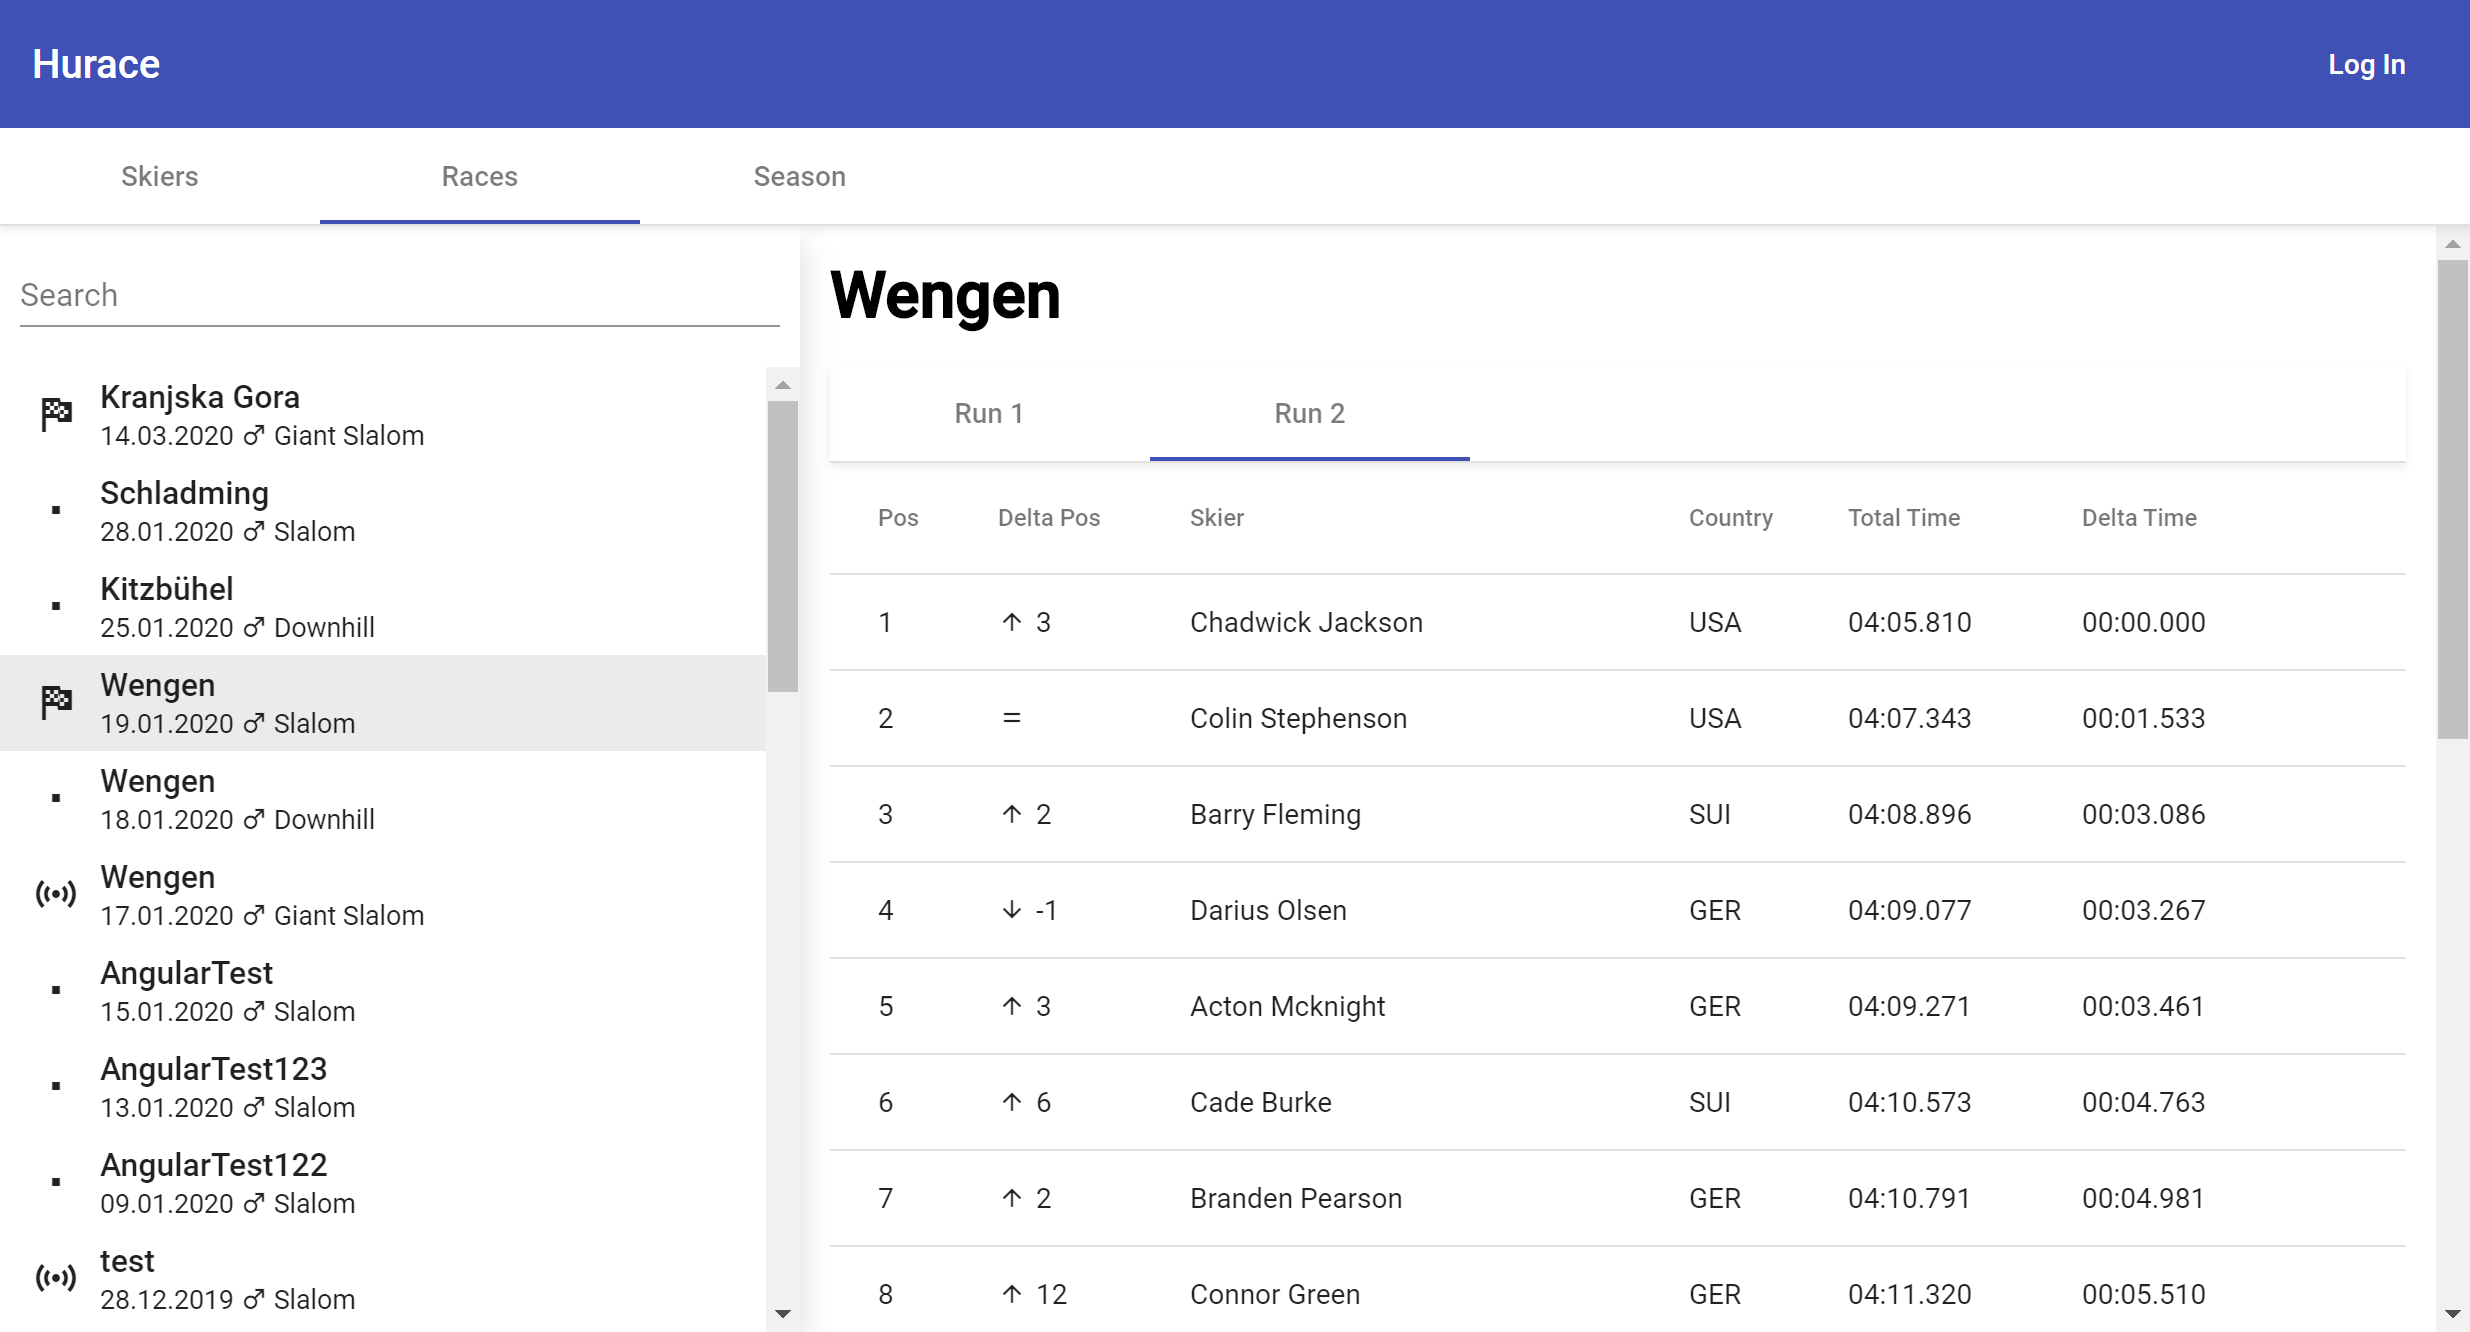
\includegraphics[width=0.9\linewidth]{images/races-detail}
    \caption{Detailansicht eines abgeschlossenen Rennens}
\label{fig:races-detail}
\end{figure}

\begin{figure}[H]
    \centering
    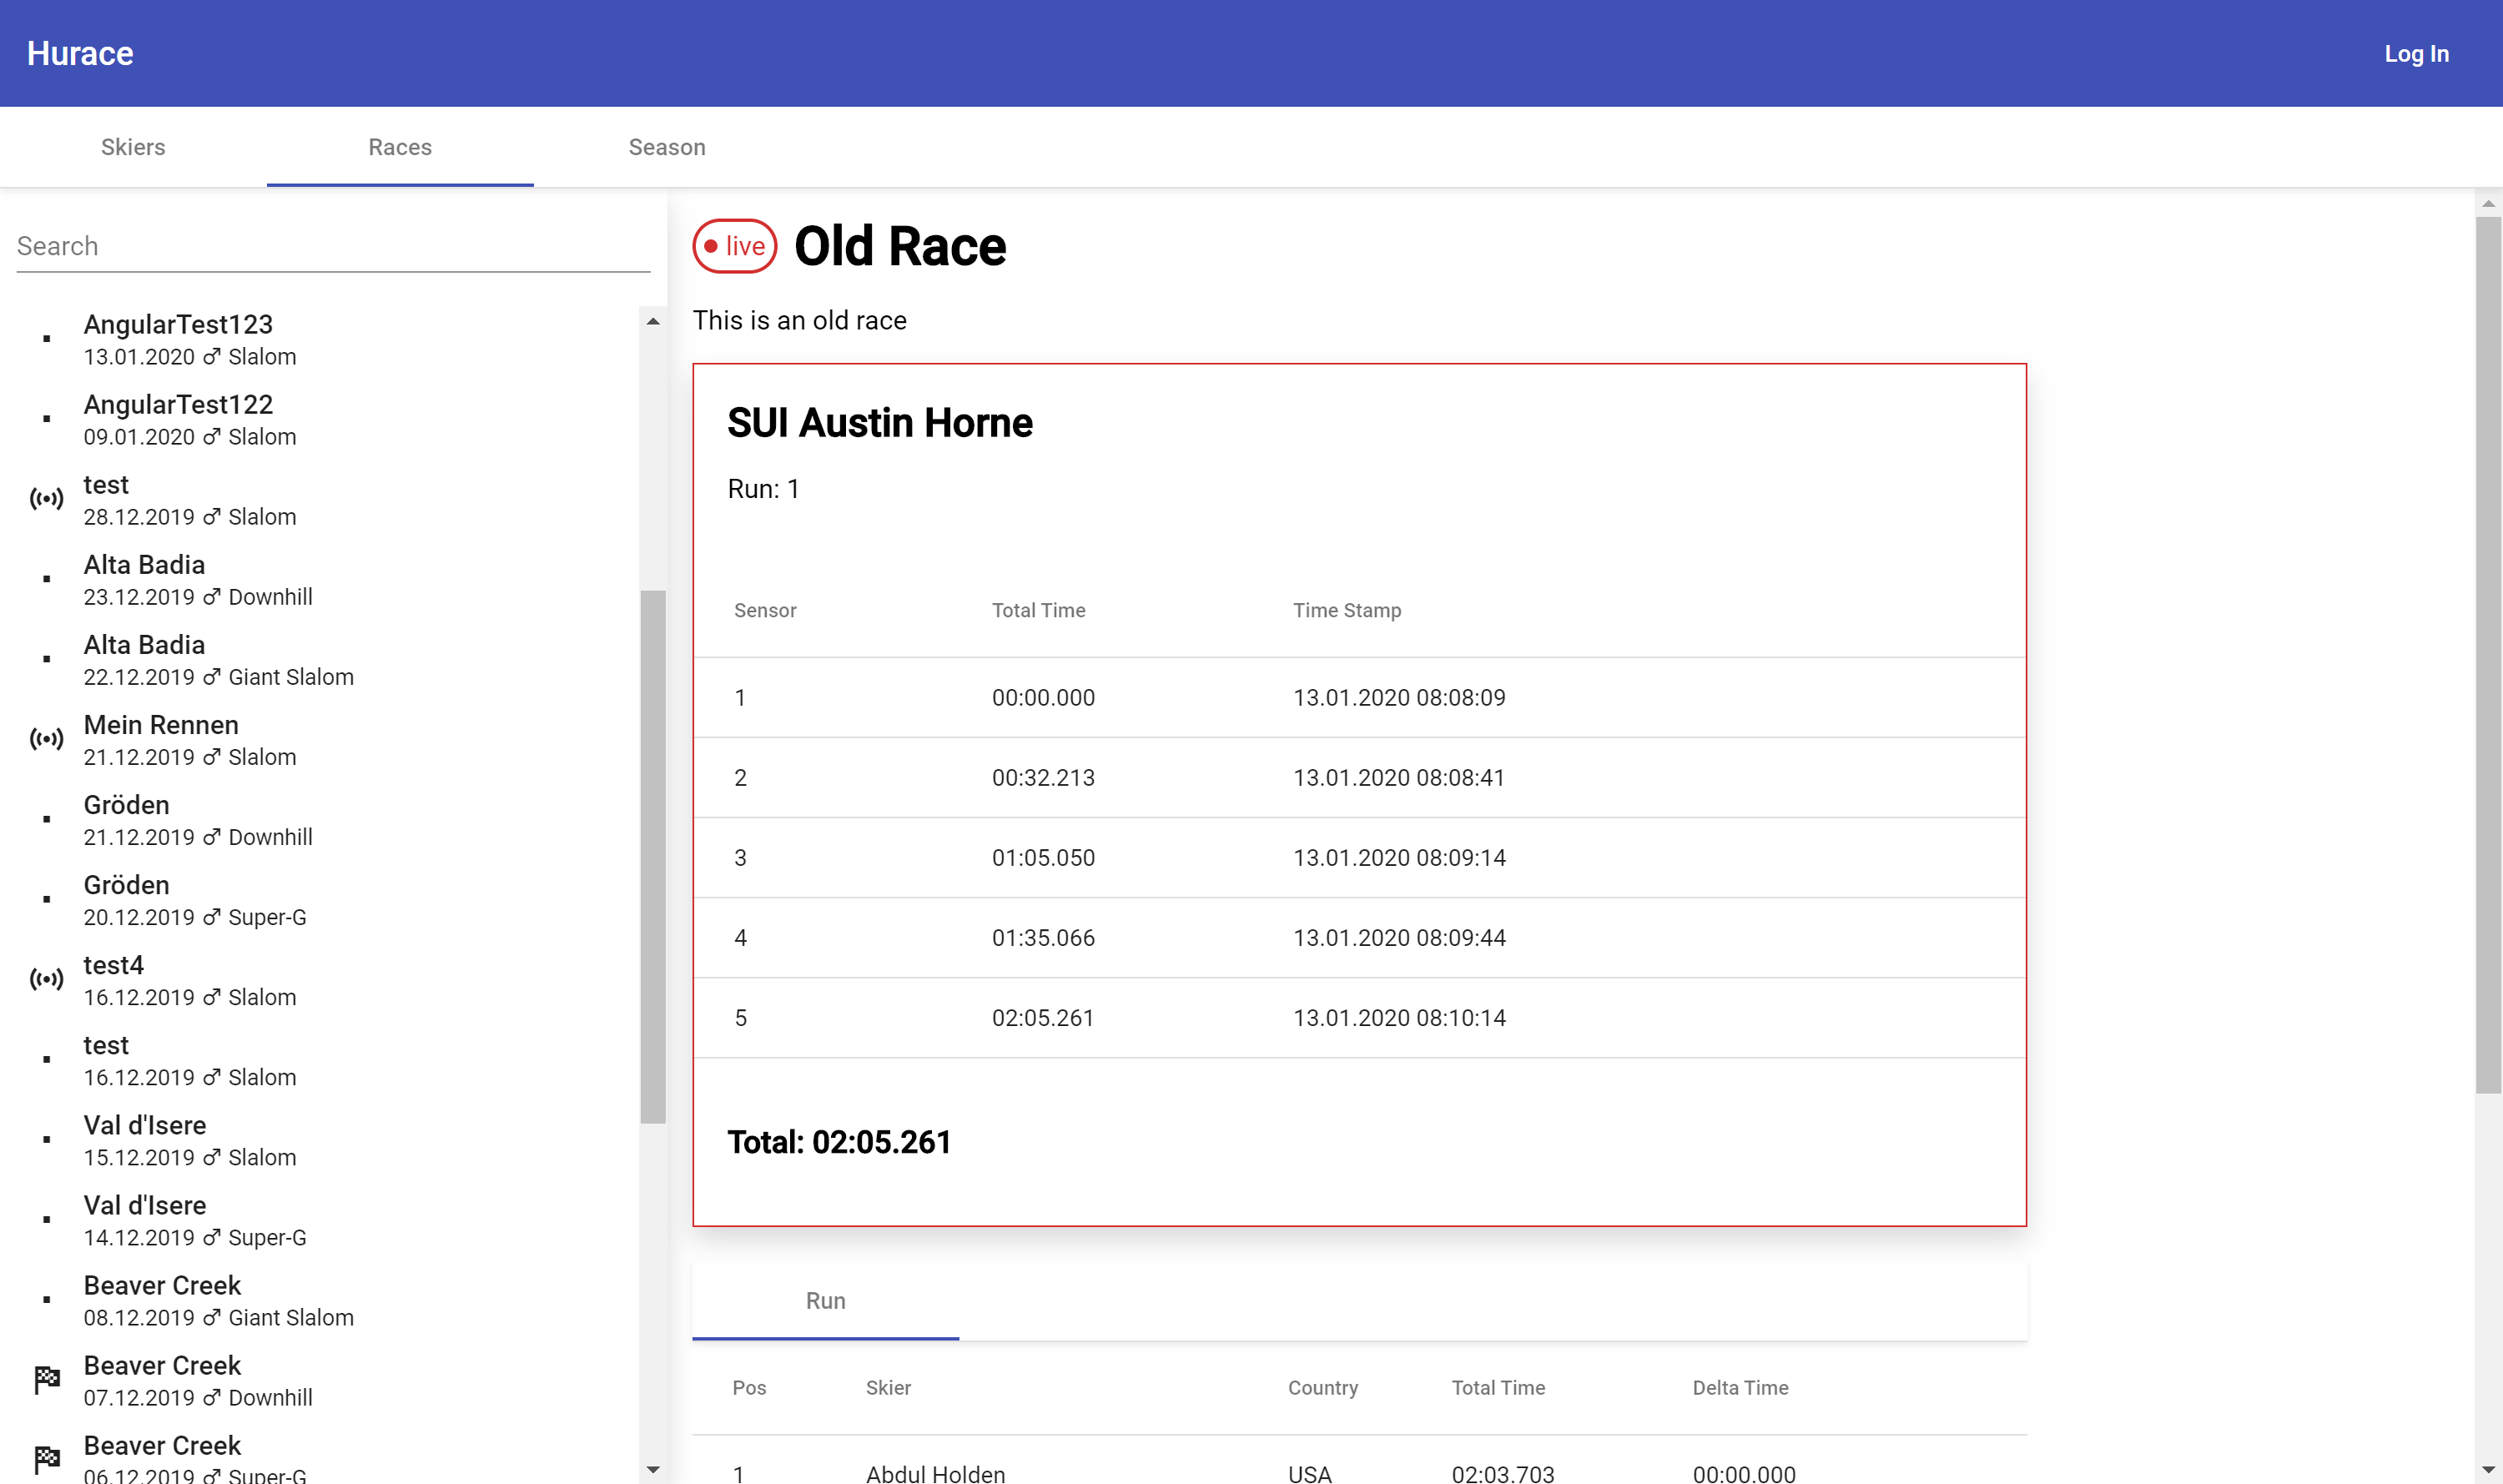
\includegraphics[width=0.9\linewidth]{images/races-live}
    \caption{Detailansicht eines laufenden Rennens}
\label{fig:races-live}
\end{figure}

\begin{figure}[H]
    \centering
    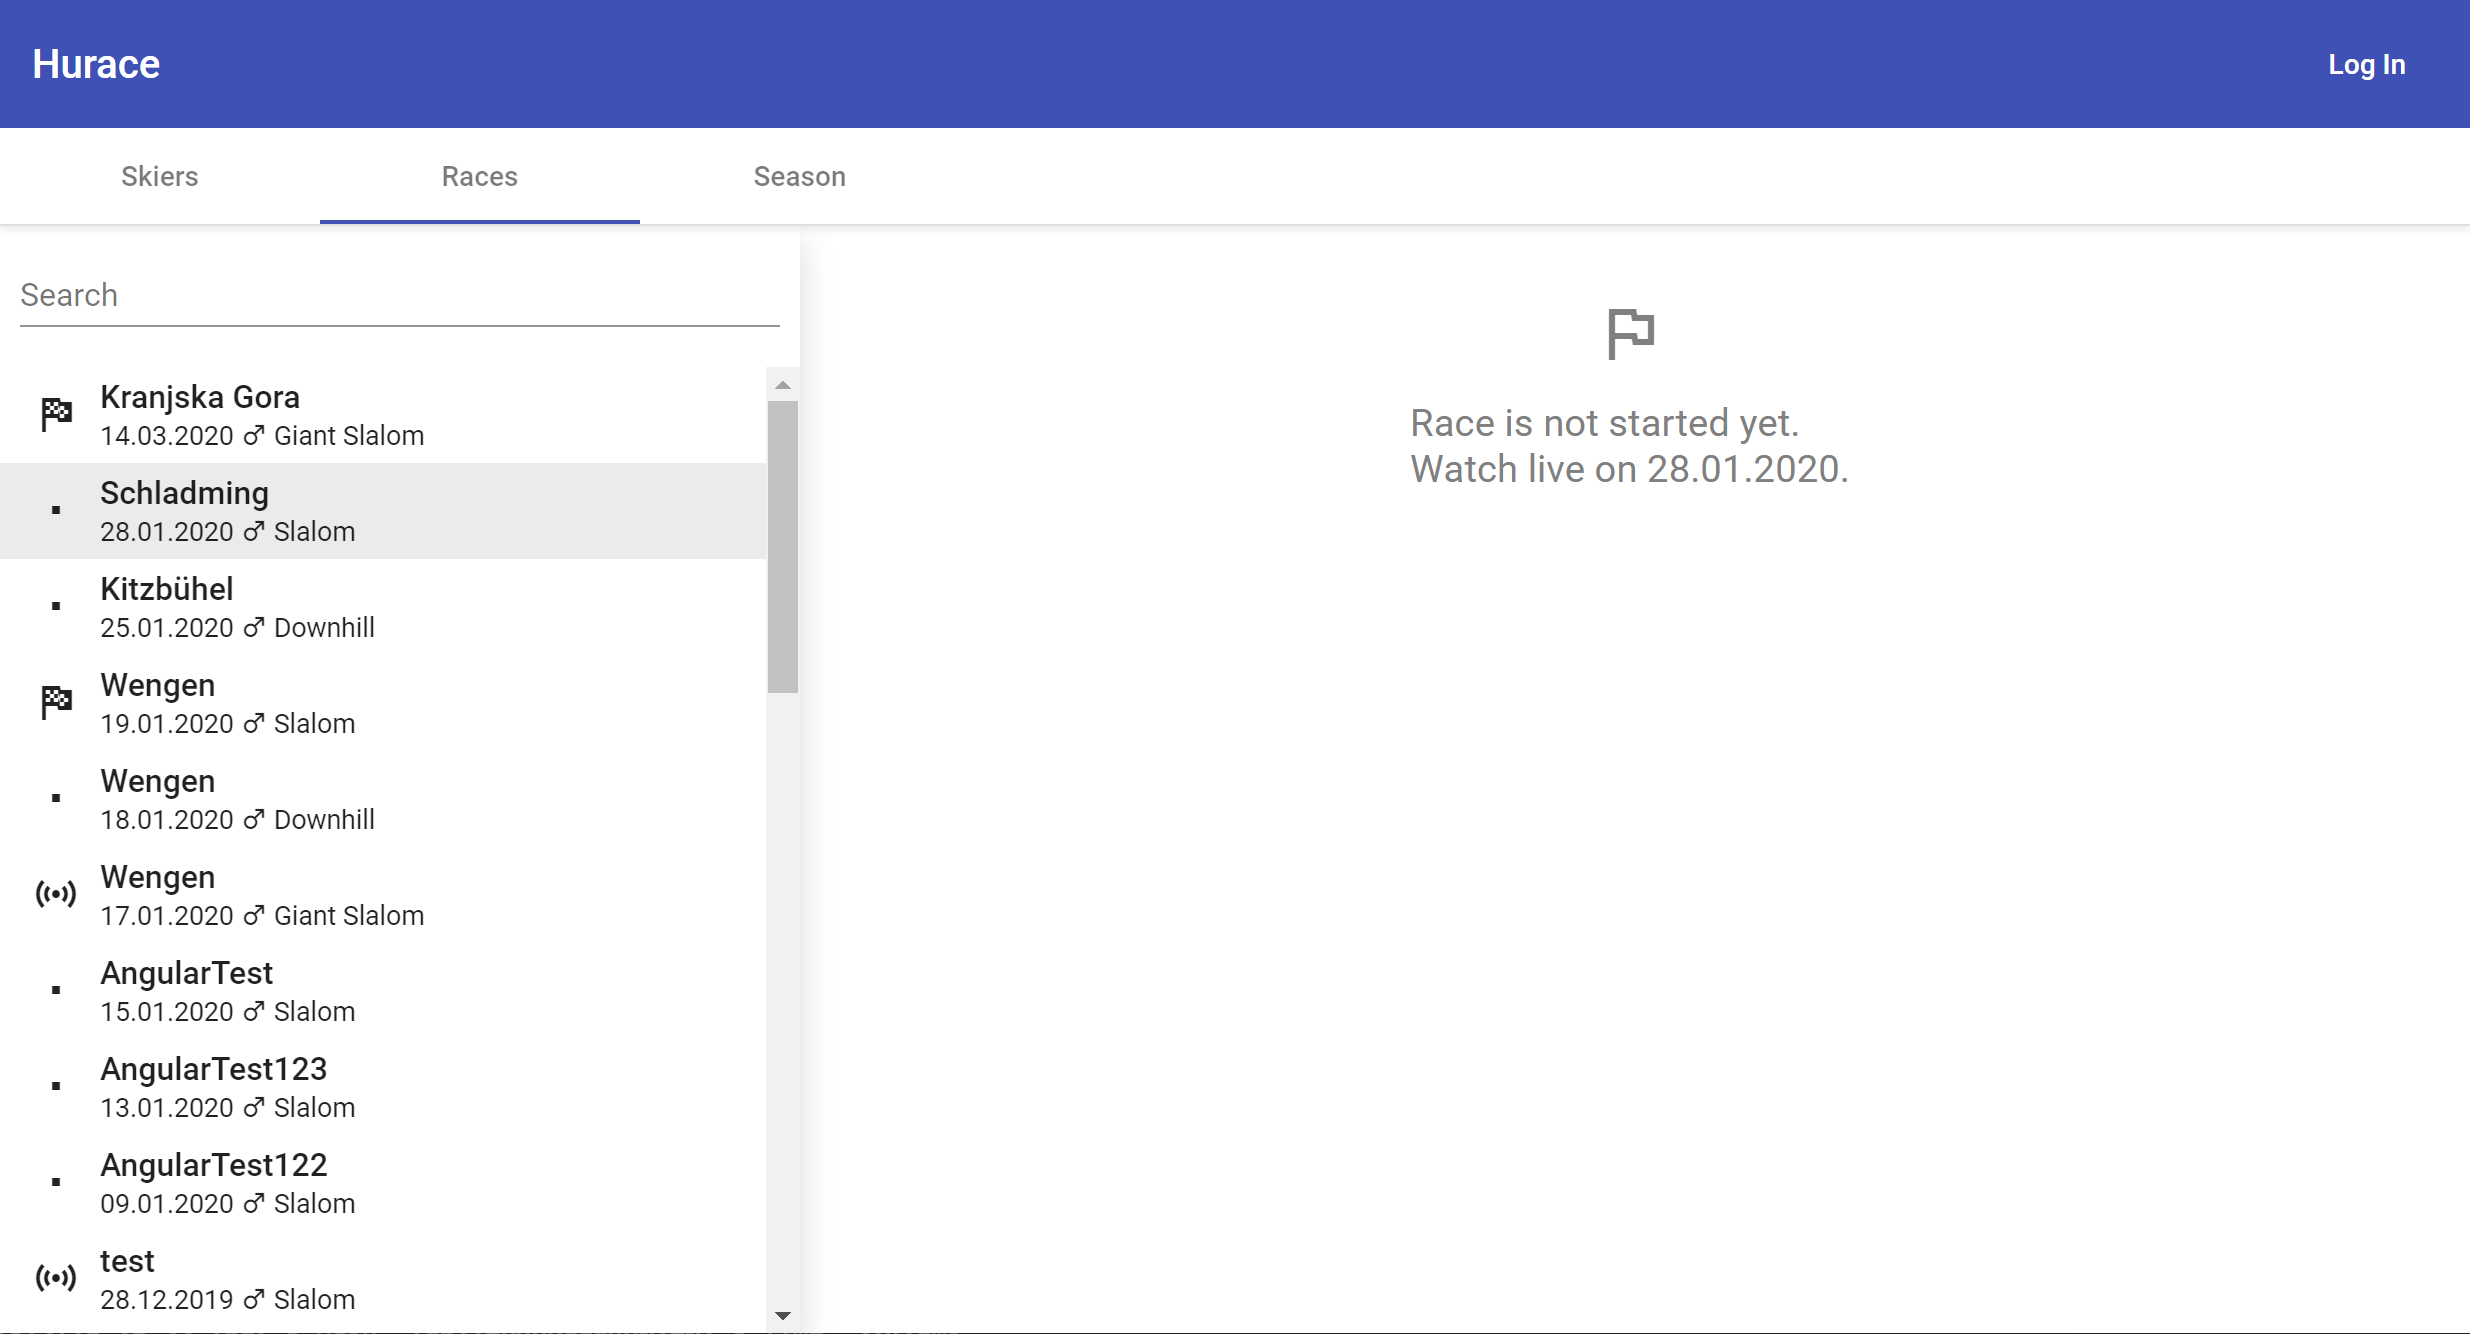
\includegraphics[width=0.9\linewidth]{images/races-not-started}
    \caption{Detailansicht eines nicht gestarteten Rennens}
\label{fig:races-not-started}
\end{figure}

\newpage
\section{Season}
Die \emph{Season}-Seite zeigt alle Rennen der aktuellen Saison nach Renntyp gegliedert an (\cref{fig:season-list}).
Mit Hilfe der Reitern (\emph{Slalom}, \emph{Giant Slalom}, \emph{Super-G} und \emph{Downhill}) kann der Renntyp gewechselt werden.
Die Liste an Rennen beinhaltet nur noch Rennen des gewählten Renntyps.
Falls ein Rennen abgeschlossen ist wird zusätzlich ein Link \emph{Show results}, der zu den Endergebnis des Rennens führt, angezeigt.
Falls ein Rennen gerade live ist wird zusätzlich ein Link \emph{Watch live}, der zu der Liveansicht des Rennens führt, angezeigt.

\begin{figure}[H]
    \centering
    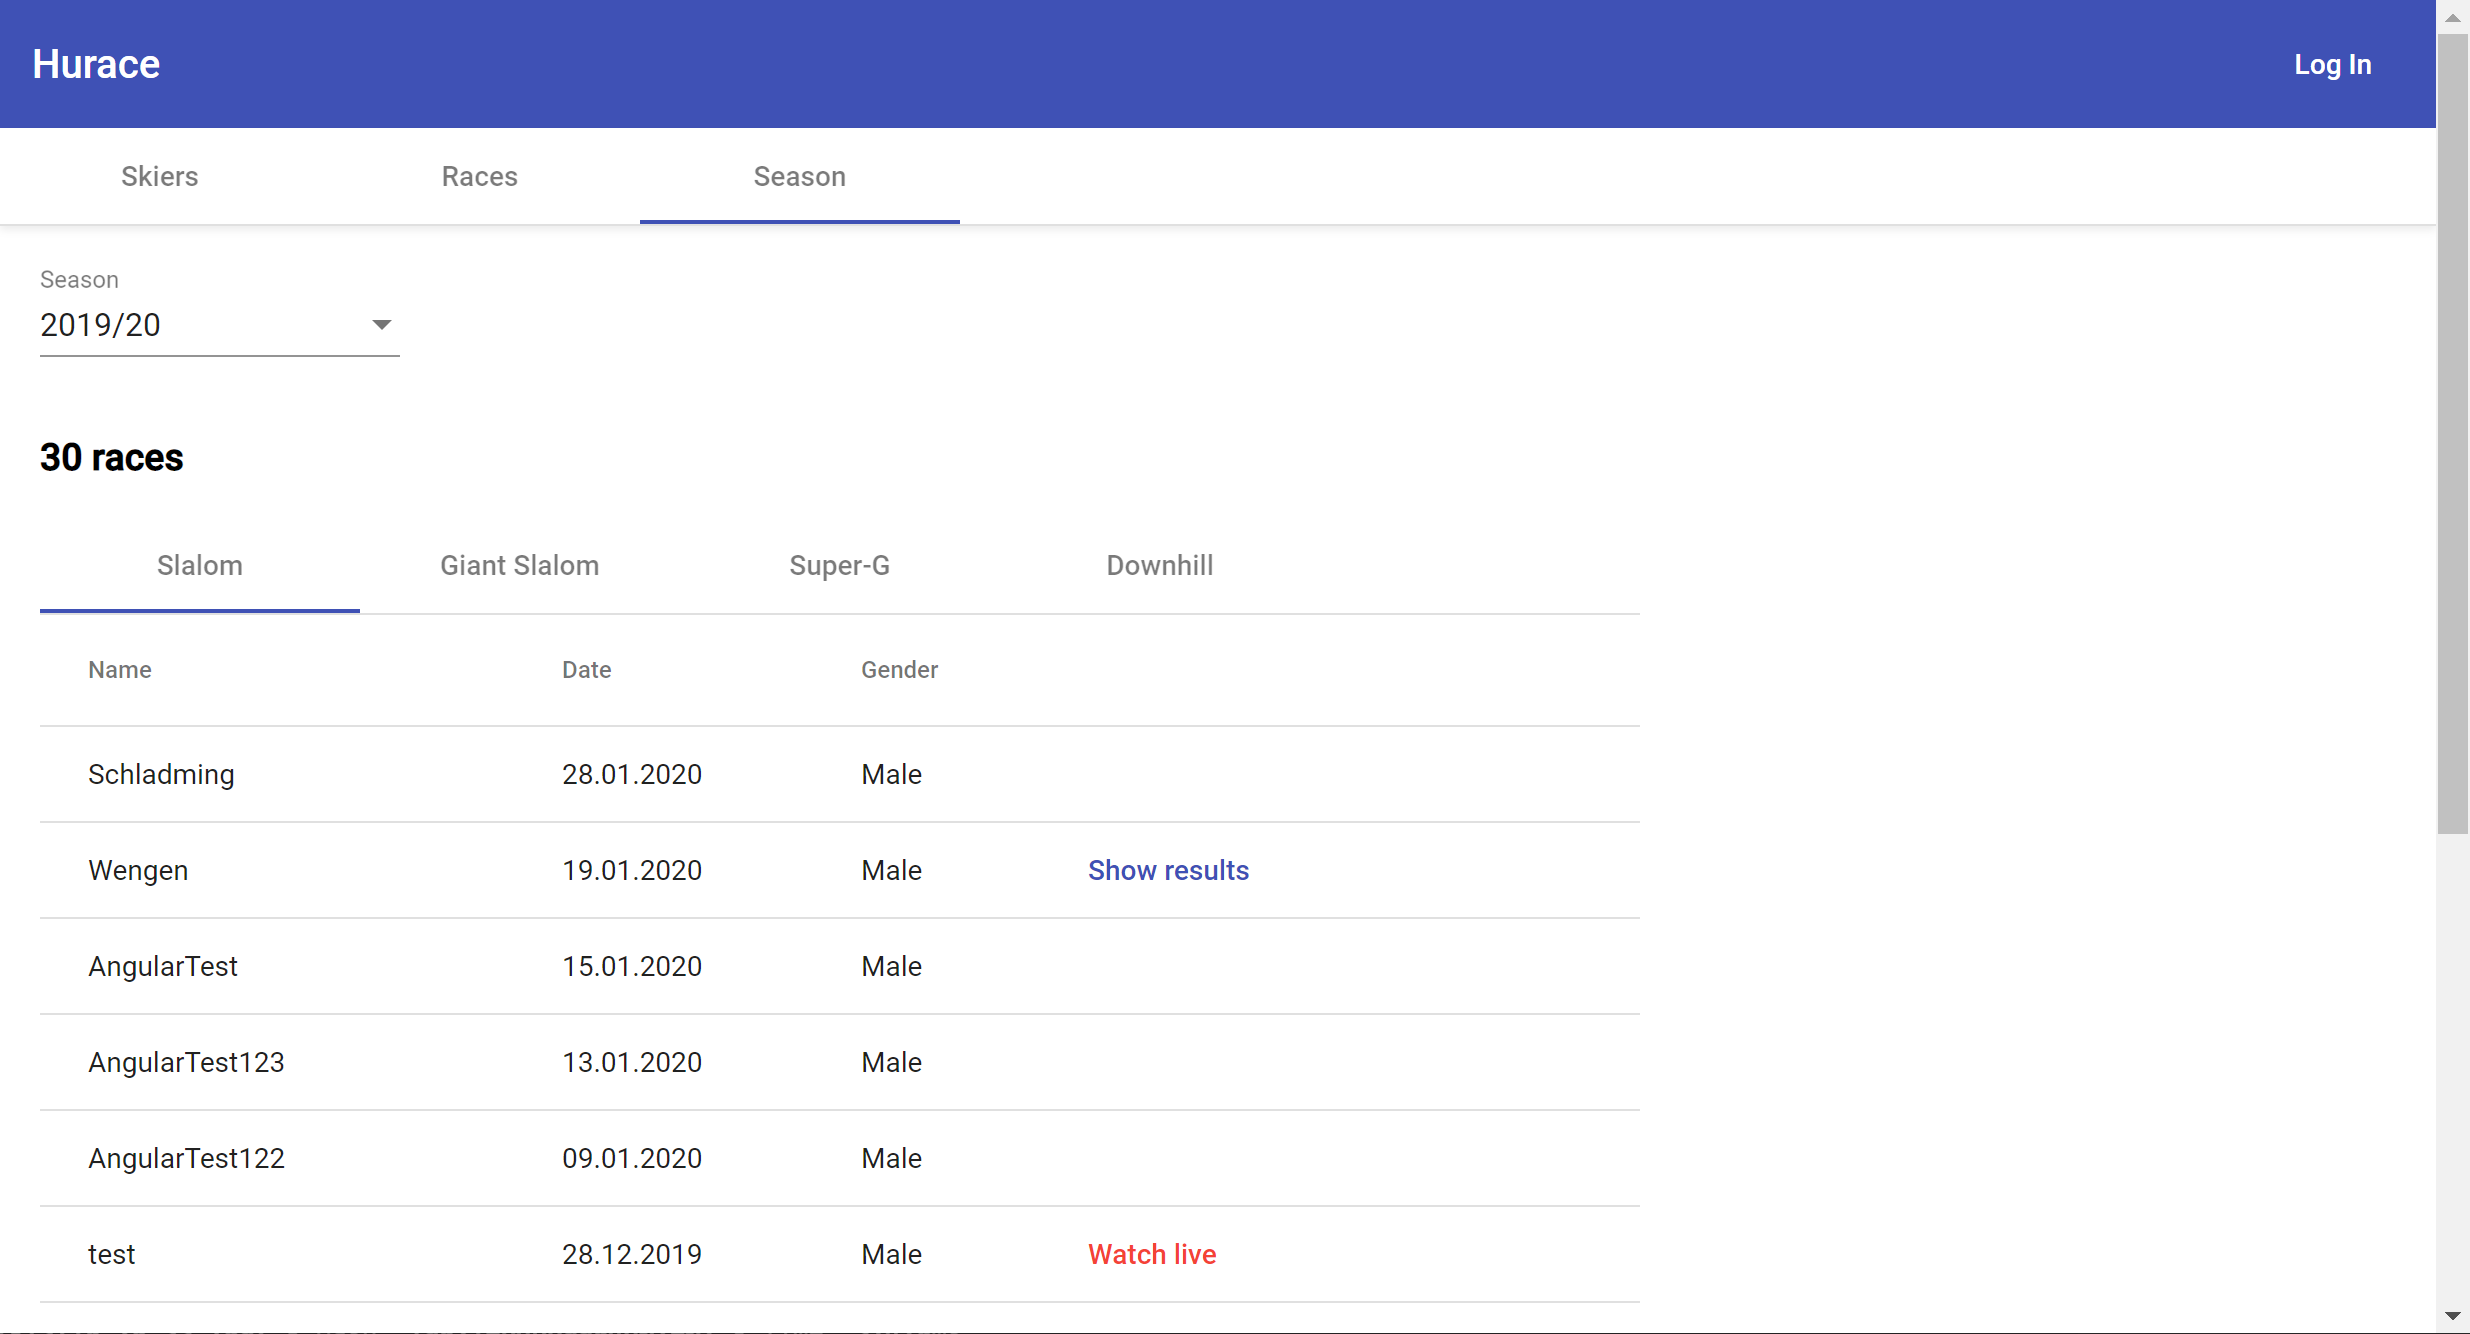
\includegraphics[width=0.9\linewidth]{images/season-list}
    \caption{Rennen nach Saison und Renntyp}
\label{fig:season-list}
\end{figure}
\listoffigures{}
\lstlistoflistings{}
\end{document}
